\chapter{Théorème de Thalès\\et transformations} \label{G11}

\bigskip

\begin{figure}[h]
   \centering
      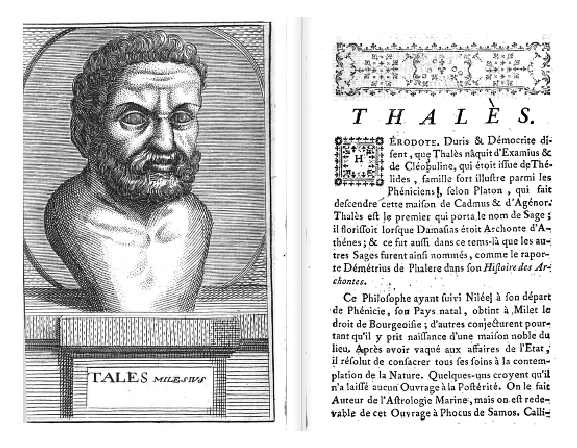
\includegraphics[height=6cm]{Geometrie/Images/G11_intro_Thales}
   \caption{Vies, doctrines et sentences des philosophes illustres, 1761, Diogenes Laertius}
\end{figure}

\bigskip

\begin{prerequis}[Un peu d'histoire]
    La tradition attribue à \textbf{Thalès de Milet} (environ $-625 ; -546$ av. J.-C.) l'introduction en Grèce de la géométrie égyptienne. Thalès n'a laissé aucun écrit, ce qui rend donc difficile la réalisation d'une biographie incontestée de ce sage. C'est un commerçant qui consacre sa vie aux voyages et aux études, philosophe et savant, il est l'auteur de nombreuses recherches mathématiques, notamment en géométrie. De retour à Milet, il devient homme politique, et homme d'affaires. Ses travaux portent sur les mathématiques, l'astrologie, l'astronomie et la philosophie. Il serait mort de déshydratation en regardant un concours gymnique, oubliant de d'alimenter et de s'hydrater.
    On dit qu’il aurait mesuré les grandes pyramides grâce à leur ombre : au cours d'un voyage en Égypte, il aperçoit la pyramide de Kheops. Les dimensions du monument âgé alors de 2 000 ans, dépassent de loin tout ce qu’il avait imaginé. \\
{\it – \og Comment mesurer cette pyramide ? \fg \\
Thalès regardant son ombre eut alors cette idée : \\
– \og Le rapport que j’entretiens avec mon ombre est le même que celui que la pyramide entretient avec la sienne. Donc, à l’instant où mon ombre sera égale à ma taille, l’ombre de la pyramide sera égale à sa hauteur. \fg} \\
    Toutefois, des documents historiques montrent que cette propriété était déjà connue bien avant par les Babyloniens et les Égyptiens. Le résultat porte le nom de Thalès en France. En anglais, il est connu sous le nom de {\it Intercept theorem} ; en allemand il est appelé {\it Strahlensatz} (théorème des rayons). La première démonstration écrite connue de ce théorème est donnée dans les {\it Éléments} d’{\bf Euclide}.
\end{prerequis}

\cours

%%%%%%%%%%%%%%%%%%%%%%%
\section{Théorème de Thalès}

\subsection{Configuration de Thalès}

\begin{propriete}[Théorème de Thalès]
   Soient $(d)$ et $(d')$ sont deux droites sécantes en $A$, $B$ et $M$ deux points de la droite $(d)$, distincts de $A$, et $C$ et $N$ deux points de la droite $(d')$, distincts de $A$. \\
   Si les droites $(BC)$ et $(MN)$ sont parallèles, alors : $\displaystyle{\frac{AM}{AB}=\frac{AN}{AC}}$.
\end{propriete}

\begin{remarque}
   ce rapport est également égal à $\dfrac{MN}{BC}$ puisque dans ce cas, les triangles $ABC$ et $AMN$ sont semblables. Autrement dit, les longueurs des côtés des triangles $ABC$ et $AMN$ sont proportionnelles.
\end{remarque}

Les trois figures clé :

{\psset{algebraic=true,unit=0.7}
\begin{pspicture}(-0.5,-2.5)(7,4)
   \psplot{-1}{5.5}{3*x/5}
   \psplot{-1}{5.5}{0}
   \psplot[linecolor=A1]{3}{5}{(17-5*x)/-2}
   \psplot[linecolor=B1]{1}{3}{(7-5*x)/-2}
   \begin{footnotesize}
      \psdots(0,0)(1.85,1.11)(4.47,2.68)(3.4,0)(1.4,0)
      \rput[bl](0,-0.4){$A$}
      \rput[bl](2,0.9){$M$}
      \rput[bl](4.6,2.4){$B$}
      \rput[bl](3.5,-0.4){$C$}
      \rput[bl](1.5,-0.4){$N$}
      \rput(6,0){$(d')$}
      \rput(6,3.5){$(d)$}
      \rput(6,-1.5){configurations \og classique \fg{}}
   \end{footnotesize}
\end{pspicture}
\begin{pspicture}(-0.5,-2.5)(7,4)
   \psplot{-1}{6}{3*x/5}
   \psplot{-1}{6}{0}
   \psplot[linecolor=A1]{3}{5}{(17-5*x)/-2}
   \psplot[linecolor=B1]{4}{6}{(22-5*x)/-2}
   \begin{footnotesize}
      \psdots(0,0)(5.8,3.5)(4.47,2.68)(3.4,0)(4.4,0)
      \rput[bl](0,-0.4){$A$}
      \rput[bl](5.8,3){$M$}
      \rput[bl](4.6,2.4){$B$}
      \rput[bl](3.5,-0.4){$C$}
      \rput[bl](4.5,-0.4){$N$}
      \rput(6.5,0){$(d')$}
      \rput(6.5,3.7){$(d)$}
   \end{footnotesize}
\end{pspicture}
\begin{pspicture}(-3.5,-2.5)(5.5,4.2)
   \psplot{-3.5}{5.5}{(-0.--3.*x)/5.}
   \psplot{-3.5}{5.5}{(-0.-0.*x)/8.}
   \psplot[linecolor=A1]{3}{5}{(--17.-5.*x)/-2.}
   \psplot[linecolor=B1]{-2.8}{-0.5}{(-9.4-5.*x)/-2.}
   \begin{footnotesize}
   \psdots(0,0)(-2.47,-1.48)(4.47,2.68)(3.4,0)(-1.88,0)
   \rput[bl](0,-0.4){$A$}
   \rput[bl](-2.23,-1.79){$M$}
   \rput[bl](4.6,2.4){$B$}
   \rput[bl](3.5,-0.4){$C$}
   \rput[bl](-1.7,-0.4){$N$}
   \rput(6,0){$(d')$}
   \rput(6,3.5){$(d)$}
   \rput(2,-2){configuration \og papillon \fg}
   \end{footnotesize}
\end{pspicture}}

\begin{preuve}
   Une démonstration parmi d'autres : le démonstration d'Euclide basée sur les aires ($-300$ avant J.-C.). \\
   \begin{minipage}{6.2cm}
   {\psset{unit=0.8}
      \begin{pspicture}(-1,-1)(7,9)
         \pspolygon(1,8)(0,0)(6,0)
         \psline(6,0)(0.25,1.94)(4.77,1.93)(0,0)
         \rput[bl](0.9,8.4){$A$}
         \rput[bl](-0.5,-0.5){$B$}
         \rput[bl](6.3,-0.5){$C$}
         \rput[bl](-0.5,1.9){$D$}
         \rput[bl](5.2,1.9){$E$}
      \end{pspicture}}
   \end{minipage}
   \begin{minipage}{9.5cm}
      Les droites (DE) et (BC) sont parallèles.
      \begin{itemize}
         \item Les triangles $DEB$ et $DEC$ on une base commune : [$DE]$ et la même hauteur donc : $\mathcal{A}(DEB) =\mathcal{A}(DEC)$ ; \\
            D'où $\mathcal{A}(ABE) =\mathcal{A}(ACD)$ par ajout de $\mathcal{A}{(ADE)}$.
         \item[\quad \, $\Longrightarrow$] \quad $\dfrac{\mathcal{A}(ABE)}{\mathcal{A}(ABC)} =\dfrac{\mathcal{A}(ACD)}{\mathcal{A}(ABC)}$ ; \\ 
         \item les triangles $ABE$ et $ABC$ ont la même hauteur issue de $B$ : $h_1$ ; \\
            les triangles $ACD$ et $ABC$ ont la même hauteur issue de $C$ : $h_2$ ;
         \item[\quad \, $\Longrightarrow$] \quad $\dfrac{\dfrac{AE\times \cancel{h_1}}{\cancel{2}}}{\dfrac{AC\times \cancel{h_1}}{\cancel{2}}} =\dfrac{\dfrac{AD\times \cancel{h_2}}{\cancel{2}}}{\dfrac{AB\times \cancel{h_2}}{\cancel{2}}}$ \\ [5pt]
         \item[\quad \, $\Longrightarrow$] \quad \fbox{$\dfrac{AE}{AC} =\dfrac{AD}{AB}$}
      \end{itemize}
   \end{minipage}
\end{preuve}

\begin{methode}[Calculer une longueur dans une configuration de Thalès]
   On utilise le théorème de Thalès en respectant la rédaction :
   \begin{itemize}
      \item citer les points alignés dans un ordre précis et les droites parallèles ;
      \item citer la propriété utilisée (\og d'après le théorème de Thalès \fg) ;
      \item écrire l'égalité des quotients ;
      \item isoler, puis calculer la longueur du segment demandé.
   \end{itemize}
   \exercice
      $ABC$ est un triangle, \\
      $M\in[AB]$, $N\in[AC]$, \\
      $AM =\ucm{5}, AN =\ucm{6}, AB =\ucm{8}$ et $BC =\ucm{4}$. \\
      Les droites $(MN)$ et $(BC)$ sont parallèles. \\
      Calculer $MN$ et $AC$.
   \correction
      {\psset{unit=0.6}
      \begin{pspicture}(-3,-2)(9,4)
         \pspolygon(0,0)(8.76,3.93)(8,0)
        \psline(5,0)(5.48,2.45)
         \rput(-0.5,0){$A$}
         \rput(5.4,-0.5){$M$}
         \rput(8,-0.5){$B$}
         \rput(5.7,3.1){$N$}
         \rput(8.75,4.5){$C$}
         \pcline[offset=-20pt,linecolor=B1]{|-|}(0,0)(8,0)
         \lput*{:U}{\textcolor{B1}{8 cm}}
         \pcline[offset=-10pt,linecolor=B1]{|-|}(0,0)(5,0)
         \lput*{:U}{\textcolor{B1}{5 cm}}
         \pcline[offset=10pt,linecolor=B1]{|-|}(0,0)(5.48,2.45)
         \lput*{:U}{\textcolor{B1}{6 cm}}
         \pcline[offset=10pt,linecolor=B1]{|-|}(8.76,3.93)(8,0)
         \lput*{:U}{\textcolor{B1}{4 cm}}
      \end{pspicture}} \\
      Les points $A, N, C$ et $A, M, B$ sont alignés dans le même ordre et les droites $(MN)$ et $(BC)$ sont parallèles. \\
      D'après le théorème de Thalès, avec des mesures en cm, on a : \\ [3pt]
      $\dfrac{AM}{AB} =\dfrac{AN}{AC} =\dfrac{MN}{BC}$ \quad soit \quad $\dfrac{5}{8} =\dfrac{6}{AC} =\dfrac{MN}{4}$ \\ [1mm]
      donc, $MN=\dfrac{5\times 4}{8} =2,5$ \quad et \quad $AC=\dfrac{6\times 8}{5}=9,6$.
\end{methode}

\bigskip


\subsection{Un cas particulier : la réciproque du théorème de la droite des milieux.} %%%

\begin{propriete}[Réciproque de la droite des milieux]
   Dans un triangle, la droite qui passe par le milieu d'un côté parallèlement à un deuxième côté coupe le troisième côté en son milieu.
\end{propriete}
   
\qquad \begin{tabular}[b]{p{0.5cm}p{6cm}p{1cm}p{5cm}}
   \bf Si
   &
   dans le triangle $ABC$, $I$ milieu de $[AB]$,
   & 
   \bf alors
   &
   $J$ milieu de $[AC]$
   \\
   & $(IJ) \ /\!/\ (BC)$ et $J \in (AC)$ & & \\
   & & & \\
   &
   {\psset{unit=1.2}
   \begin{pspicture}(-1,-0.3)(3,2)
      \psline(0,0)(1,2)(3,0)
      \put(-0.4,-0.4){$B$}
      \put(3.2,-0.4){$C$}
      \put(0.9,2.2){$A$}
      \put(0.2,1.1){$I$}
      \put(2.1,1.1){$J$}
      \rput(0.25,0.5){\textcolor{A1}{$\sim$}}
      \rput(0.75,1.5){\textcolor{A1}{$\sim$}}
      \psline[linecolor=B1](-0.5,1)(3.5,1)
      \psline[linecolor=B1](-0.5,0)(3.5,0)
   \end{pspicture}}
   & &
   {\psset{unit=1.2}
   \begin{pspicture}(0,-0.3)(3,2)
      \pspolygon(0,0)(3,0)(1,2)
      \put(-0.4,-0.4){B}
      \put(3.2,-0.4){\textcolor{A1}{$C$}}
      \put(0.9,2.2){\textcolor{A1}{ $A$}}
      \put(0.2,1.1){I}
      \put(2.1,1.1){\textcolor{A1}{ $J$}}
      \rput(1.5,1.5){\textcolor{A1}{$\equiv$}}
      \rput(2.5,0.5){\textcolor{A1}{$\equiv$}}
      \psline(0.5,1)(2,1)
   \end{pspicture}}
\end{tabular}

\begin{preuve}
   $A, I, B$ et $A, J, C$ sont alignés dans le même ordre et $(IJ)$ est parallèle à $(BC)$, donc d'après le théorème de Thalès, $\dfrac{AI}{AB} = \dfrac{AJ}{AC}$. \\ [1mm]
   Or, $I$ est le milieu de $[AB]$, d'où $\dfrac{AI}{AB} =\dfrac12$, donc $\dfrac{AJ}{AC} =\dfrac12$ ce qui implique que $AJ =\dfrac12AC$.
\end{preuve}


%%%%%%%%%%%%%%%%%%%%%%%%%%
\section{Réciproque du théorème de Thalès}


\subsection{Configuration de Thalès, sens réciproque}

\begin{propriete}[Réciproque du théorème de Thalès]
   Si les points $A$, $M$ et $B$ d'une part, et les points $A$, $N$ et $C$ d'autre part, sont alignés dans le même ordre, et si les rapports $\dfrac{AM}{AB}$ et $\dfrac{AN}{AC}$ sont égaux, alors les droites $(MN)$ et $(BC)$ sont parallèles.
\end{propriete}

\begin{methode*2*2}[Démontrer que deux droites sont parallèles]
   On utilise le théorème de Thalès en respectant la rédaction :
   \begin{itemize}
      \item citer les points alignés dans un ordre précis ;
      \item calculer deux rapports de longueur ; \\
      \parbox[t]{0.49\linewidth}{
         {\bf s'il y a égalité}
         \begin{itemize}
            \item écrire l'égalité ;
            \item citer la propriété utilisée : \og d'après la réciproque du théorème de Thalès \dots \fg{};
            \item conclure : \og les droites \dots{} et \dots{} sont parallèles \fg
         \end{itemize}  
      }\hfill\vrule\hfill
      \parbox[t]{0.49\linewidth}{
         {\bf s'il n'y a pas égalité}
         \begin{itemize}
            \item écrire l'inégalité ;
            \item citer la propriété utilisée : \og d'après la contraposée au théorème de Thalès\dots \fg{};
            \item conclure : \og les droites \dots{} et \dots{} ne sont pas parallèles \fg
         \end{itemize}}
   \end{itemize}
   \exercice
      $A\in[NC]$ et $A\in [MB]$. \\
      $AM=5$, $AN=6$, $AB=7,5$ et $AC=9$. \\
      Les droites $(MN)$ et $(BC)$ sont-elles parallèles ?
   \correction    
      \begin{center}
      {\psset{unit=0.5}
         \begin{pspicture}(-5,-3.5)(8,5)
            \pspolygon(-5,0)(7.5,0)(7.8,4.5)(-5.2,-3)
            \rput(0,0.35){$A$}
            \rput(-5.5,0){$M$}
            \rput(8,0){$B$}
            \rput(-5.5,-3.5){$N$}
            \rput(8.2,4.8){$C$}
            \pcline[offset=10pt,linecolor=B1]{|-|}(-5,0)(-0.1,0)
            \lput*{:U}{\textcolor{B1}{5}}
            \pcline[offset=-10pt,linecolor=B1]{|-|}(-5.2,-3)(-0.1,0)
            \lput*{:U}{\textcolor{B1}{6}}
            \pcline[offset=-10pt,linecolor=B1]{|-|}(0.1,0)(7.5,0)
            \lput*{:U}{\textcolor{B1}{7,5}}
            \pcline[offset=10pt,linecolor=B1]{|-|}(0.1,0)(7.8,4.5)
           \lput*{:U}{\textcolor{B1}{9}}
         \end{pspicture}}
      \end{center}
      Les points $M$, $A$ , $B$ d'une part, et les points $N$, $A$, $C$ d'autre part, sont alignés dans le même ordre. \\
      On calcule $\dfrac{AM}{AB} =\dfrac{5}{7,5} =\dfrac{2}{3}$ \quad d'une part, \\
      et \quad $\dfrac{AN}{AC} =\dfrac{6}{9} =\dfrac{2}{3}$ \quad d'autre part. \\  
      On constate que $\dfrac{AM}{AB} =\dfrac{AN}{AC}$; \\ [1mm]
      d'après la réciproque du théorème de Thalès, les droites $(MN)$ et $(BC)$ sont parallèles.
   \exercice
      $M\in[AB]$, $N\in[AC]$, \\
      $AM =\ucm{5}, AN =\ucm{6}, AB =\ucm{8}, AC =\ucm{9}$. \\
      Les droites $(MN)$ et $(BC)$ sont-elles parallèles ?
   \correction
      \begin{center}
      {\psset{unit=0.7}
        \begin{pspicture}(-1,-1.25)(9,3.25)
            \pspolygon(0,0)(8.5,3)(8,0)
            \psline(5,0)(5.66,2)
            \rput(-0.5,0){$A$}
            \rput(5.4,-0.5){$M$}
            \rput(8.5,0){$B$}
            \rput(5.9,2.5){$N$}
            \rput(8.8,3.3){$C$}
            \pcline[offset=-20pt,linecolor=B1]{|-|}(0,0)(8,0)
            \lput*{:U}{\textcolor{B1}{\ucm{8}}}
            \pcline[offset=-10pt,linecolor=B1]{|-|}(0,0)(5,0)
            \lput*{:U}{\textcolor{B1}{\ucm{5}}}
            \pcline[offset=10pt,linecolor=B1]{|-|}(0,0)(5.66,2)
            \lput*{:U}{\textcolor{B1}{\ucm{6}}}
            \pcline[offset=20pt,linecolor=B1]{|-|}(0,0)(8.5,3)
            \lput*{:U}{\textcolor{B1}{\ucm{9}}}
         \end{pspicture}}
      \end{center}
      Les points $A, N, C$ et $A, M, B$ sont alignés dans le même ordre. \\
      On calcule $\dfrac{AM}{AB} =\dfrac{5}{8}$ \quad d'une part, \\
      et $\dfrac{AN}{AC} =\dfrac{6}{9} =\dfrac{2}{3}$ \quad d'autre part. \\  
      On constate que $\dfrac{AM}{AB}\neq\dfrac{AN}{AC}$ ; \\ [1mm]
      or, si les droites $(MN)$ et $(BC)$ étaient parallèles, le théorème de Thalès nous dirait que cette égalité est vraie. Comme ce n'est pas le cas, on peut en conclure que les droites $(MN)$ et $(BC)$ ne sont pas parallèles.
\end{methode*2*2}


\subsection{Un cas particulier : le théorème de la droite des milieux.}

\begin{propriete}[Théorème de la droite des milieux]
   Dans un triangle, la droite qui joint les milieux de deux côtés est parallèle au troisième côté et la longueur du segment qui joint les milieux de ces deux côtés est égale à la moitié de la longueur du troisième côté.
\end{propriete}

\begin{tabular}[b]{p{0.5cm}p{5cm}p{1.5cm}p{3cm}p{1cm}p{3cm}}
   \bf Si
   &
   dans le triangle $ABC$, $I$ milieu de $[AB]$ et $J$ milieu de $[AC]$.
   & 
   \bf alors
   &
   $(IJ)\, \ /\!/\ \,(BC)$
   &
  \bf et
   &
   $IJ=\displaystyle{\frac12}BC$
   \\ 
   & & & & & \\    
   &
   \begin{pspicture}(-1,0.2)(3,2)
      \pspolygon(0,0)(3,0)(1,2)
      \put(-0.4,-0.2){$B$}
      \put(3.2,-0.2){$C$}
      \put(0.9,2.2){$A$}
      \put(0.2,1){\textcolor{A1}{$I$}}
      \put(2.1,1){\textcolor{A1}{$J$}}
      \rput(0.25,0.5){\textcolor{A1}{$\sim$}}
      \rput(0.75,1.5){\textcolor{A1}{$\sim$}}
      \rput(1.5,1.5){\textcolor{A1}{$\equiv$}}
      \rput(2.5,0.5){\textcolor{A1}{$\equiv$}}
      \psline(0.5,1)(2,1)
   \end{pspicture}
   &
   &
   \begin{pspicture}(0,0.2)(3,2)
      \psline(0,0)(1,2)(3,0)
      \put(-0.4,-0.4){$B$}
      \put(3.2,-0.4){$C$}
      \put(0.9,2.2){$A$}
      \put(0.2,1.1){$I$}
      \put(2.1,1.1){$J$}
      \psline[linecolor=B1](-0.5,1)(3.5,1)
      \psline[linecolor=B1](-0.5,0)(3.5,0)
   \end{pspicture}
   & &
   \begin{pspicture}(0,0.2)(3,2)
      \psline(0,0)(1,2)(3,0)
      \put(-0.4,-0.2){$B$}
      \put(3.2,-0.2){$C$}
      \put(0.9,2.2){$A$}
      \put(0.2,1){$I$}
      \put(2.1,1){$J$}
      \psline[linecolor=B1]{|-|}(0.5,1)(2,1)
      \rput(1.25,0.7){\textcolor{B1}{$\frac12BC$}}
      \psline{|-|}(0,0)(3,0)
   \end{pspicture}
   \\
\end{tabular}

\begin{preuve}
   $A, I, B$ et $A, J, C$ sont alignés dans le même ordre. \\
   $I$ est le milieu de $[AB]$ et $J$ est le milieu de $[AC]$, d'où $\dfrac{AI}{AB} =\dfrac12$ et $\dfrac{AJ}{AC} =\dfrac12$. \\
   $\dfrac{AI}{AB} =\dfrac{AJ}{AC}$, d'après la réciproque du théorème de Thalès, les droites $(IJ)$ et $(BC)$ sont parallèles. \\ [1mm]
   De plus, $\dfrac{AI}{AB} =\dfrac{AJ}{AC} =\dfrac{IJ}{BC}$ ce qui implique que $\dfrac{IJ}{BC} =\dfrac12$, soit $IJ =\dfrac12BC$.
\end{preuve}


%%%%%%%%%%%%%%%%%%%%%
\section{Les transformations}

\subsection{Isométries et homothéties}

\begin{definition}[Isométrie, homothétie]
   Une \textbf{isométrie} est une transformation qui conserve les longueurs. \\
   Une \textbf{homothétie} est une transformation qui réduit ou qui agrandit une figure .
\end{definition}

\begin{propriete}
   \begin{itemize}
      \item Deux triangles sont {\bf isométriques} (ou égaux) s'il sont superposables et deux triangles sont {\bf semblables} si leurs côtés sont proportionnels, ou s'ils ont les mêmes angles.
      \item Une isométrie {\bf conserve} les longueurs, le parallélisme, l'orthogonalité, les angles, les formes et les figures.
      \item Dans la configuration de Thalès, l'un des triangles est image de l'autre par une {\bf homothétie} dont le centre est le sommet commun et le rapport est donné par le rapport de Thalès.
      \item Une {\bf homothétie} de rapport $k$ multiplie les aires par $k^2$ et les volumes par $k^3$. \\ [-8mm]
   \end{itemize}
 \end{propriete}
 
\begin{exemple*1}
   Exemples de triangles isométriques. \\
   {\psset{unit=0.35}
   \hspace*{0.2cm}
      \begin{pspicture}(0,-2)(10,6.7) 
         \psline[linecolor=B1](1,0)(5,2)
         \psline[linecolor=J1](2,5)(5,2)
         \psline[linecolor=A1](1,0)(2,5)
         \psline[linecolor=B1](6,3)(10,1)
         \psline[linecolor=J1](6,3)(9,6)
         \psline[linecolor=A1](10,1)(9,6)
         \rput(0.7,-0.3){\footnotesize{$A$}}
         \rput(5.3,1.7){\footnotesize{$B$}}
         \rput(1.8,5.3){\footnotesize{$C$}}
         \rput(10.3,0.7){\footnotesize{$A'$}}
         \rput(5.7,2.7){\footnotesize{$B'$}}
         \rput(9.3,6.3){\footnotesize{$C'$}}
         \rput(5.5,-1.7){\parbox{4.5cm}{trois côtés de même longueur}}  
      \end{pspicture}
   \hspace*{1.3cm}
      \begin{pspicture}(0,-2)(10,6.7)   
         \psline(1,0)(5,2)
         \psline[linecolor=A1](2,5)(5,2)
         \psline[linecolor=B1](1,0)(2,5)
         \psline(6,3)(10,1)
         \psline[linecolor=A1](6,3)(9,6)
         \psline[linecolor=B1](10,1)(9,6)
         \rput(0.7,-0.3){\footnotesize{$A$}}
         \rput(5.3,1.7){\footnotesize{$B$}}
         \rput(1.8,5.3){\footnotesize{$C$}}
         \rput(10.3,0.7){\footnotesize{$A$'}}
         \rput(5.7,2.7){\footnotesize{$B$'}}
         \rput(9.3,6.3){\footnotesize{$C$'}}
         \SpecialCoor
         \pswedge[fillstyle=solid,fillcolor=J1](2,5){1}{(-1,-5)}{(1,-1)}
         \pswedge[fillstyle=solid,fillcolor=J1](9,6){1}{(-1,-1)}{(1,-5)}
        \rput(5.4,-2.3){\parbox{4.5cm}{un angle égal compris entre deux côtés de même longueur}}
      \end{pspicture}
   \hspace*{1.3cm}
      \begin{pspicture}(0,-2)(8,6.7)
         \psline(1,0)(5,2)
         \psline(2,5)(5,2)
         \psline[linecolor=B1](1,0)(2,5)
         \psline(6,3)(10,1)
         \psline(6,3)(9,6)
         \psline[linecolor=B1](10,1)(9,6)
         \rput(0.7,-0.3){\footnotesize{$A$}}
         \rput(5.3,1.7){\footnotesize{$B$}}
         \rput(1.8,5.3){\footnotesize{$C$}}
         \rput(10.3,0.7){\footnotesize{$A$'}}
         \rput(5.7,2.7){\footnotesize{$B$'}}
         \rput(9.3,6.3){\footnotesize{$C$'}}
         \SpecialCoor
         \pswedge[fillstyle=solid,fillcolor=J1](2,5){1}{(-1,-5)}{(1,-1)}
         \pswedge[fillstyle=solid,fillcolor=J1](9,6){1}{(-1,-1)}{(1,-5)}
         \pswedge[fillstyle=solid,fillcolor=A1](1,0){1}{(2,1)}{(1,5)}
         \pswedge[fillstyle=solid,fillcolor=A1](10,1){1}{(-1,5)}{(-2,1)}
         \rput(5.4,-2.3){\parbox{4.5cm}{un côté de même longueur adjacent à deux angles égaux}}
      \end{pspicture}}
\end{exemple*1}


\subsection{Les symétries} %%%%%%

\begin{definition}[Symétrie axiale]
   $M'$ est l'image du point $M$ par la \textbf{symétrie d'axe $\Delta$} signifie que la droite $\Delta$ est la médiatrice du segment $[MM']$. C'est une isométrie.
\end{definition}
   
\begin{center}
   {\psset{unit=0.75}
   \begin{pspicture}(-4,-0.2)(4,3.5)
      \pstGeonode[PointName=none, PointSymbol=none](0,-0.5){O}(0,3.5){O'}
      \pstLineAB{O}{O'}
      \pstTriangle[PosAngleA=115](1,1){A}(4,0){B}(2,3){C}
      \psset{CodeFig=true, CodeFigColor=A1, linecolor=B1, RightAngleSize=0.2}
      \pstOrtSym[SegmentSymbol=pstslash, PosAngle=50]{O}{O'}{A}
      \pstOrtSym[SegmentSymbol=pstslashh, PosAngle=-135]{O}{O'}{B}
      \pstOrtSym[SegmentSymbol=pstslashhh, PosAngle=90]{O}{O'}{C}
      \pstLineAB[linecolor=B1]{A'}{B'}
      \pstLineAB[linecolor=B1]{B'}{C'}
      \pstLineAB[linecolor=B1]{C'}{A'}
      \rput(0,3.8){$\Delta$}
   \end{pspicture}}
\end{center}

On dit que les figures sont symétriques par rapport à la droite $\Delta$.

\begin{definition}[Symétrie centrale]
   $M'$ est l'image du point $M$ par la \textbf{symétrie de centre $O$} signifie que $O$ est le milieu de $[MM']$. C'est une isométrie.
\end{definition}

\begin{center}
   {\psset{unit=0.75}
   \begin{pspicture}(-4,-0.2)(4,3.25)
      \pstGeonode[PosAngle=-90](0,1.5){O}
      \pstTriangle(1,0){A}(4,0){B}(2,2){C}
      \pstSymO[CodeFig=true, CodeFigColor=A1, PosAngle={40,170,-90}]{O}{A, B, C}[A', B', C']
      \pstLineAB[linecolor=B1]{A'}{B'}
      \pstLineAB[linecolor=B1]{C'}{B'}
      \pstLineAB[linecolor=B1]{A'}{C'}
   \end{pspicture}}
\end{center}

\begin{definition}[Axe, centre de symétrie]
   Si une figure $\cal F$ est \og{}transformée\fg{} en elle-même par la symétrie axiale d'axe (d), alors la droite (d) est un \textbf{axe de symétrie} de la figure $\cal F$. \\
   Si une figure $\cal F$ est \og{}transformée\fg{} en elle-même par la symétrie centrale de centre O, alors O est le \textbf{centre de symétrie} de la figure $\cal F$.
\end{definition}

\begin{exemple*1}
   Une figure peut avoir plusieurs axes de symétrie mais si elle possède un centre de symétrie il est unique.
   {\psset{unit=0.75}
   \begin{multicols}{3}
      \begin{center}
         \begin{pspicture}(-2.5,0)(2.5,2)
            \pstGeonode[PointName=none,PointSymbol=none,CurveType=polygon](-1,0){A}(1,0){B}(0,2){C}
            \pstGeonode[PointName=none,PointSymbol=none,CurveType=polygon,linecolor=B1](0,-0.5){D}(0,2.5){E}
      \end{pspicture}
   
      \textbf{triangle isocèle} \\
      1 axe de symétrie \\
      0 centre de symétrie \\    
      \begin{pspicture}(-2.5,0)(2.5,2)
         \pstGeonode[PointName=none,PointSymbol=none,CurveType=polygon](-1.156,0){A}(1.156,0){B}(0,2){C}
         \pstGeonode[PointName=none,PointSymbol=none,CurveType=polygon,linecolor=B1](0,-0.5){D}(0,2.5){E}
         \psline[linecolor=B1](-1.156,0)(2;50)
         \psline[linecolor=B1](1.156,0)(2;130)
      \end{pspicture}
   
      \textbf{triangle équilatéral} \\
      3 axes de symétrie \\
      0 centre de symétrie \\  
      \begin{pspicture}(-2.5,0)(2.5,2)
         \pscircle(0,1){1}
         \psset{linecolor=B1}
         \psline(-1.5,1)(1.5,1)
         \psline(0,-0.5)(0,2.5)
         \psline(-1.5,-0.5)(1.5,2.5)
         \psline(-1.5,2.5)(1.5,-0.5)
         \psline(-0.5,-0.5)(0.5,2.5)
         \psline(-0.5,2.5)(0.5,-0.5)
         \psline(-1.5,0)(1.5,2)
         \psline(-1.5,0.5)(1.5,1.5)
         \psline(-1.5,2)(1.5,0)
         \psline(-1.5,1.5)(1.5,0.5)  
         \psdot[linecolor=A1,linewidth=1mm](0,1)   
      \end{pspicture}
   
      \textbf{cercle} \\
      $\infty$ axes de symétrie \\
      1 centre de symétrie  
   \end{center}
\end{multicols}

\begin{multicols}{3}
   \begin{center}
      \begin{pspicture}(-2.5,0)(2.5,2)
         \pspolygon(-1,0)(1,0)(1,2)(-1,2)
         \psset{linecolor=B1}
         \psline(-1.5,1)(1.5,1)
         \psline(0,-0.5)(0,2.5)
         \psline(-1.5,-0.5)(1.5,2.5)
         \psline(-1.5,2.5)(1.5,-0.5)
         \psdot[linecolor=A1,linewidth=1mm](0,1)
      \end{pspicture}
      
      \textbf{carré} \\
      4 axes de symétrie \\
      1 centre de symétrie \\
      \begin{pspicture}(-2.5,0)(2.5,2)
         \pspolygon(-1.5,0)(1.5,0)(1.5,2)(-1.5,2)
         \psset{linecolor=B1}
         \psline(-2,1)(2,1)
         \psline(0,-0.5)(0,2.5)
         \psdot[linecolor=A1,linewidth=1mm](0,1)  
      \end{pspicture}
   
      \textbf{rectangle} \\
      2 axes de symétrie \\
      1 centre de symétrie \\ 
      \begin{pspicture}(-2.5,0)(2.5,2)
         \pspolygon(-1.5,0)(1,0)(1.5,2)(-1,2)
         \psset{linecolor=A1,linewidth=1mm}
         \psdot(0,1)  
      \end{pspicture}
   
      \textbf{parallélogramme}  \\
      0 axe de symétrie \\
      1 centre de symétrie
      \end{center}
   \end{multicols}}
\ \\ [-1.5cm]
\end{exemple*1}


\subsection{Les rotations} %%%

\begin{definition}[Rotation]
   $M'$ est l'image du point $M$ par la \textbf{rotation de centre $O$ et d'angle $\alpha$} signifie que $OM=OM'$ et que $\widehat{MOM'} =\alpha$. C'est une isométrie.
\end{definition}
 
\begin{center}
   \begin{pspicture}(-3,-0.25)(5,3.75)
      \psset{arrowscale=1.7}
      \pstGeonode[PosAngle=-90](0,0){O}
      \pstGeonode[CurveType=polygon](2,0){M}(5,0){N}(5,1.5){P}(4,2){Q}
     \pstRotation[RotAngle=135,CodeFig=true,CodeFigColor=A1,TransformLabel=\alpha]{O}{M}[M']
     \pstRotation[RotAngle=135,PosAngle=180]{O}{P}[P']
     \pstRotation[RotAngle=135]{O}{N}[N']
     \pstRotation[RotAngle=135,PosAngle=180]{O}{Q}[Q']
     \pstLineAB[linecolor=B1]{M'}{N'}
     \pstLineAB[linecolor=B1]{N'}{P'}
     \pstLineAB[linecolor=B1]{P'}{Q'}
     \pstLineAB[linecolor=B1]{Q'}{M'}
   \end{pspicture}
\end{center}

\begin{remarque}
   on appelle sens direct le sens inverse des aiguilles d'une montre et sens indirect le sens horaire.
\end{remarque}

 
\subsection{Les translations} %%%

\begin{definition}[Translation]
   Un point $C$ est l'mage d'un point $D$ par la \textbf{translation} qui transforme $A$ en $B$ lorsque le quadrilatère $ABCD$ est un parallélogramme. On dit alors que $C$ est l'image du point $D$ par la translation de \textbf{vecteur} $\overrightarrow{AB}$. C'est une isométrie correspondant à un déplacement.
\end{definition}

\begin{remarque}
   pour la translation de vecteur $\overrightarrow{AB}$ transformant $D$ en $C$, on a : \\
   \begin{minipage}{9cm}
   \begin{itemize}
      \item $(AB)$ et $(DC)$ sont parallèles (même direction) ;
      \item $AB$ et $DC$ sont de même longueur ;
      \item $\overrightarrow{AB}$ et $\overrightarrow{DC}$ vont dans le même sens. \\
   \end{itemize}
   Les vecteurs sont souvent notés $\overrightarrow{u}, \overrightarrow{v}$\dots
\end{minipage}
\qquad
\begin{minipage}{6cm}
   \begin{pspicture}(5,4.5)
   {\psset{arrowscale=2,unit=0.8}
      \psgrid[gridlabels=0,subgriddiv=0,griddots=10](6,5)
      \psline[linecolor=A1]{|->}(1,1)(4,2)
      \rput(0.8,0.8){$A$}
      \rput(4.2,1.8){$B$}
      \psline[linecolor=A1]{|->}(2,3)(5,4)
      \rput(1.8,3.2){$D$}
      \rput(5.2,4.2){$C$}
      \psline(1,1)(2,3)
      \psline[linecolor=B1](4,2)(5,4)
      \rput(2.6,1.2){\textcolor{A1}{$\overrightarrow{u}$}}
      \rput(3.1,3){\textcolor{A1}{$\overrightarrow{u}$}}}
   \end{pspicture}
\end{minipage}
\end{remarque}

\begin{center}
   {\psset{unit=0.7}
   \begin{pspicture}(-1,-1.5)(13,5)
      \pstGeonode[PosAngle={0,180,0,180,0}](2,-1){A}(0,0){B}(3,1){C}(-2,3){D}(3,4){E}
      \pstGeonode[PosAngle=-90](10,-2){O}
      \psset{CodeFig=true, CodeFigColor=A1}
      \pstTranslation{A}{O}{A}
      \pstTranslation[PosAngle=180]{A}{O}{B}
      \pstTranslation{A}{O}{C}
      \pstTranslation[PosAngle=180]{A}{O}{D}
      \pstTranslation{A}{O}{E}
      \pstLineAB{A}{B}
      \pstLineAB{B}{C}
      \pstLineAB{C}{D}
      \pstLineAB{D}{E}
      \pstLineAB[linecolor=B1]{A'}{B'}
      \pstLineAB[linecolor=B1]{B'}{C'}
      \pstLineAB[linecolor=B1]{C'}{D'}
      \pstLineAB[linecolor=B1]{D'}{E'}
      \rput(7,4){\textcolor{A1}{$\overrightarrow{u} =\overrightarrow{AO}$}}
   \end{pspicture}}
\end{center}


%%%%%%%%%%%%%%%%%%%%%%%%%%%%%%%%
%%%%%%%%%%%%%%%%%%%%%%%%%%%%%%%%
\activites

%%%
\begin{activite}[Groupement 3 - Exercice 3 - Question 2 : Thalès et aire]
   \ \\ [-16mm]
   \begin{QCM}
      Une enseignante a le projet d’installer un potager \uline{rectangulaire} $ADEF$ sur une parcelle de forme triangulaire $ABC$ dans l’enceinte de l’école. \\
      Les points $A, B, C, D, E$ et $F$ sont tels que :
      \begin{itemize}
         \item $AB =\um{24}$, $AC =\um{10}$ et $BC =\um{26}$ ;
         \item $D\in[AB], E\in[BC]$ et $F\in[AC]$.
      \end{itemize}
      \begin{center}
         \small
         \psset{yunit=1.3}
            \begin{pspicture}(-1,-0.3)(12,5.5)     
               \rput{10}(0,0){\pstGeonode[PointSymbol=none,CurveType=polygon,PosAngle={-135,10,100},PointName={A,B,C}]{S}(12,0){R}(0,5){C}
               \psframe[fillstyle=vlines](0,0)(2,4.17)
               \rput(2,-0.3){$D$}
               \rput(-0.3,4.17){$F$}
               \rput(2.2,4.5){$E$}}
            \end{pspicture} \\
            {\it La figure ci-dessus n'est pas à l'échelle.} \smallskip
      \end{center}
      On souhaite déterminer où positionner le point $D$ sur $[AB]$ pour que l’aire du rectangle hachuré $ADEF$ soit la plus grande possible. \\
      Dans cette partie on considère que $AD =4,8$ m.
      \begin{enumerate}
         \item Montrer que la longueur $DE$ est égale 8 m.
         \item En déduire l’aire du rectangle $ADEF$ en m$^2$. \medskip
      \end{enumerate}
   \end{QCM}
   
   \bigskip
   
   \textcolor{G1}{
   {\bf Exemple de corrigé.}
      \begin{enumerate}
         \item $ADEF$ est un rectangle, les côtés $(AF)$ et $(DE)$ sont donc parallèles. \\
            De plus, les points $B, D, A$ et $B, E, C$ sont alignés dans cet ordre. \\ [1mm]
            D'après le théorème de Thalès : $\dfrac{BD}{BA} =\dfrac{BE}{BC} =\dfrac{DE}{AC} \iff \dfrac{\um{24}-\um{4,8}}{\um{24}} =\dfrac{BE}{\um{26}} =\dfrac{DE}{\um{10}}$ \\ [1.5mm]
            \hspace*{7.5cm} $\Longrightarrow\dfrac{\um{19,2}}{\um{24}} =\dfrac{DE}{\um{10}}$ \\ [1.5mm]
            \hspace*{7.5cm} $\Longrightarrow DE =\dfrac{\um{19,2}\times\um{10}}{\um{24}} =\um{8}$. \\
            \uline{La longueur $DE$ est égale à 8 m}.
         \item $\mathcal{A}_{ADEF} =AD\times DE =\um{4,8}\times\um{8} =\umq{38,4}$. \\
            \uline{L'aire du triangle $ADEF$ est égale à \umq{38,4}}. \\
      \end{enumerate}}
      
   {\it Remarque : la question 3. suivante reprend cette question dans laquelle la longueur $AD$ est égale à $x$. Elle a été traitée dans le chapitre N3 \og Calcul littéral \fg.}
\end{activite}


%%%%%%%%%%%%%%%%%%%%%%%%%%%%%%%%
%%%%%%%%%%%%%%%%%%%%%%%%%%%%%%%%
\exercicesbase

\begin{center}
   {\cursive Maîtriser les bases avec} \href{http://mathenpoche.sesamath.net}{
\includegraphics[width=3cm]{Nombres_et_calculs/Images/mathenpoche}} \\
   \bigskip
   {\hautab{0.85}
   \cursive
   \begin{Ltableau}{0.775\linewidth}{4}{C{1}|C{1}|p{7cm}|p{2.3cm}}
      \hline
      Classe & \texttt{N\degre} & Thème & Dans le cours \\
      \hline
      \textcolor{orange}{\bf 6\up{e}} & \texttt{E5} & Symétrie axiale & 3. \\
      \hline
      \textcolor{cyan}{\bf 5\up{e}} & \texttt{D2} & Transformation et parallélogramme & 3. \\
      \hline
      \textcolor{violet}{\bf 4\up{e}} & \texttt{D2} & Transformation et parallélogramme & 3. \\
      & \texttt{D4} & Triangles et proportionnalité & 1. et 2. \\
      \hline
      \textcolor{teal}{\bf 3\up{e}} & \texttt{D2} & transformations & 3. \\
      & \texttt{D4} & Triangles et proportionnalité & 1. et 2. \\
      \hline
  \end{Ltableau}}
\end{center}

\bigskip

\begin{exercice}[DNB 2002 et CRPE 2020 G3] %%%1
   \begin{minipage}[t]{0.5\linewidth}
      Les deux parties suivantes sont indépendants. \\ [5mm]
      {\bf Partie 1}. \\
      Ce pavage est composé de 18 pentagones tous \\
      superposables. \\
      Quatre d'entre eux ont été numérotés. \\ [3mm]
      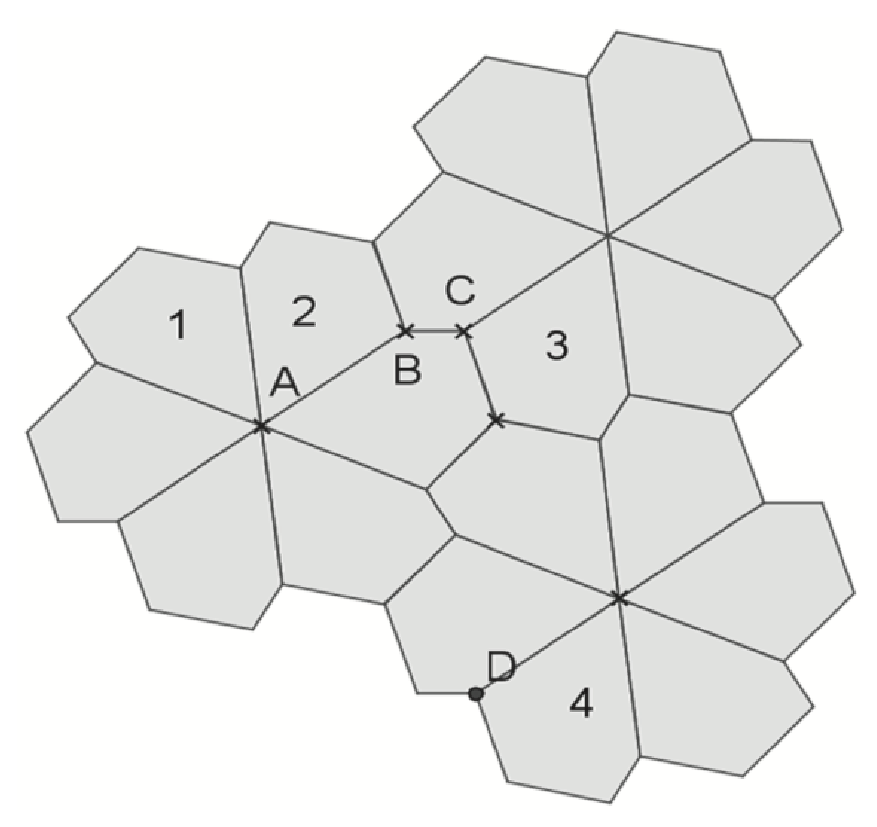
\includegraphics[width=7.5cm]{Geometrie/Images/G11_ex_transformations} \\ [3mm]
      Indiquer quelle transformation (translation, rotation, \\
      symétrie) permet de passer :
      \begin{enumerate}
         \item du pentagone 1 au pentagone 2 ;
         \item du pentagone 2 au pentagone 3 ;
         \item du pentagone 3 au pentagone 4.
      \end{enumerate}
      Préciser dans chaque cas les éléments qui définissent \\
      la transformation choisie. \\
      Aucune justification n'est attendue.
   \end{minipage}
   \begin{minipage}[t]{0.5\linewidth}
      {\bf Partie 2}. \\
      Sur le quadrillage ci-dessous :
      \begin{enumerate}
         \item tracer le symétrique $\mathcal{P}_1$ de la figure $\mathcal{P}$ \\
            par rapport au point O ;
         \item tracer le symétrique $\mathcal{P}_2$ de la figure $\mathcal{P}$ \\
            par rapport à la droite (EF) ; 
         \item tracer l'image $\mathcal{P}_3$ de la  figure $\mathcal{P}$ \\
            par la translation de vecteur $\overrightarrow{\text{AB}}$ ;
         \item tracer l'image $\mathcal{P}_4$ de la figure $\mathcal{P}$ dans la rotation \\
            de centre E, d'angle \udeg{90} dans le sens direct. \smallskip
      \end{enumerate}
      {\psset{unit=0.58cm}
      \begin{pspicture}(1,0)(15,18)
         \psgrid[gridlabelcolor=white,subgriddiv=1]
         \psline(1,0)(15,14)
         \pspolygon[linewidth=1.5pt](3,7)(4,8)(6,8)(7,9)(6,10)(5,10)(4,9)(3,10)
         \psline[linewidth=1.5pt]{->}(3,13)(5,17)
         \psdots(8,9)(7,6)(12,11)
         \uput[dr](5,9){$\mathcal{P}$}
         \uput[ul](8,9){O}
         \uput[dr](7,6){E}
         \uput[ul](3,13){A}
        \uput[ul](5,17){B}
         \uput[ul](12,11){F }    
      \end{pspicture}
      }
   \end{minipage}
\end{exercice}

\begin{corrige}
   {\bf Partie 1}. \\
   \begin{enumerate}
      \item Pour passer du polygone 1 au polygone 2, on effectue {\blue la rotation de centre A et d'angle \udeg{60} dans le sens indirect}.
      \item Pour passer du polygone 2 au polygone 3, on effectue {\blue la symétrie dont le centre est le milieu de [BC]}.
      \item Pour passer du polygone 3 au polygone 4, on effectue {\blue la translation de vecteur $\overrightarrow{CD}$, ou qui transforme le point $C$ en le point $D$}. \bigskip
   \end{enumerate}
   {\bf Partie 2}. \\
   {\psset{unit=0.58}
   \begin{pspicture}(-5,0)(18,17.5)
      \psgrid[subgriddiv=1,gridlabelcolor=white](1,0)(15,18)
      \psline(1,0)(15,14)
      \pspolygon[linewidth=1.5pt](3,7)(4,8)(6,8)(7,9)(6,10)(5,10)(4,9)(3,10)
      \psline[linewidth=1.5pt]{->}(3,13)(5,17)
      \uput[dr](5,9){$\mathcal{P}$}
      \psdots(8,9)(7,6)(12,11)
      \uput[ul](8,9){O}
      \uput[ul](3,13){A}
      \uput[ul](5,17){B}  
      \uput[dr](7,6){E}
      \uput[ul](12,11){F }    
      \pspolygon[linewidth=1.5pt,linecolor=B2](13,11)(12,10)(10,10)(9,9)(10,8)(11,8)(12,9)(13,8)
      \uput[dr](10,9){\textcolor{B2}{$\mathcal{P}_1$}} %P1
      \pspolygon[linewidth=1.5pt,linecolor=A1](8,2)(9,3)(9,5)(10,6)(11,5)(11,4)(10,3)(11,2)
      \uput[dr](9,5){\textcolor{A1}{$\mathcal{P}_2$}} %P2
      \pspolygon[linewidth=1.5pt,linecolor=blue](5,11)(6,12)(8,12)(9,13)(8,14)(7,14)(6,13)(5,14)
      \uput[dr](7,13){\textcolor{blue}{$\mathcal{P}_3$}} %P3
      \pspolygon[linewidth=1.5pt,linecolor=violet](6,2)(5,3)(5,5)(4,6)(3,5)(3,4)(4,3)(3,2)  
      \uput[dr](4,5){\textcolor{violet}{$\mathcal{P}_4$}} %P4
   \end{pspicture}}
\end{corrige}

\bigskip


\begin{exercice}[Une conjecture à démontrer] %%%2
   ABC est un triangle et $M$ est le milieu du côté $[BC]$. $R$ est un point qui décrit la médiane $[AM]$. Par $R$, on trace les parallèles à $(AB)$ et à $(AC)$ ; elles coupent le segment $[BC]$ en $D$ et $E$.
   \begin{enumerate}
      \item Faire une figure avec un logiciel de géométrie dynamique et afficher les longueurs $MD$ et $ME$.
      \item Déplacer le point $R$. Que peut-on conjecturer pour $MD$ et $ME$ ?
      \item Démontrer cette conjecture.   
   \end{enumerate}

\begin{center}
      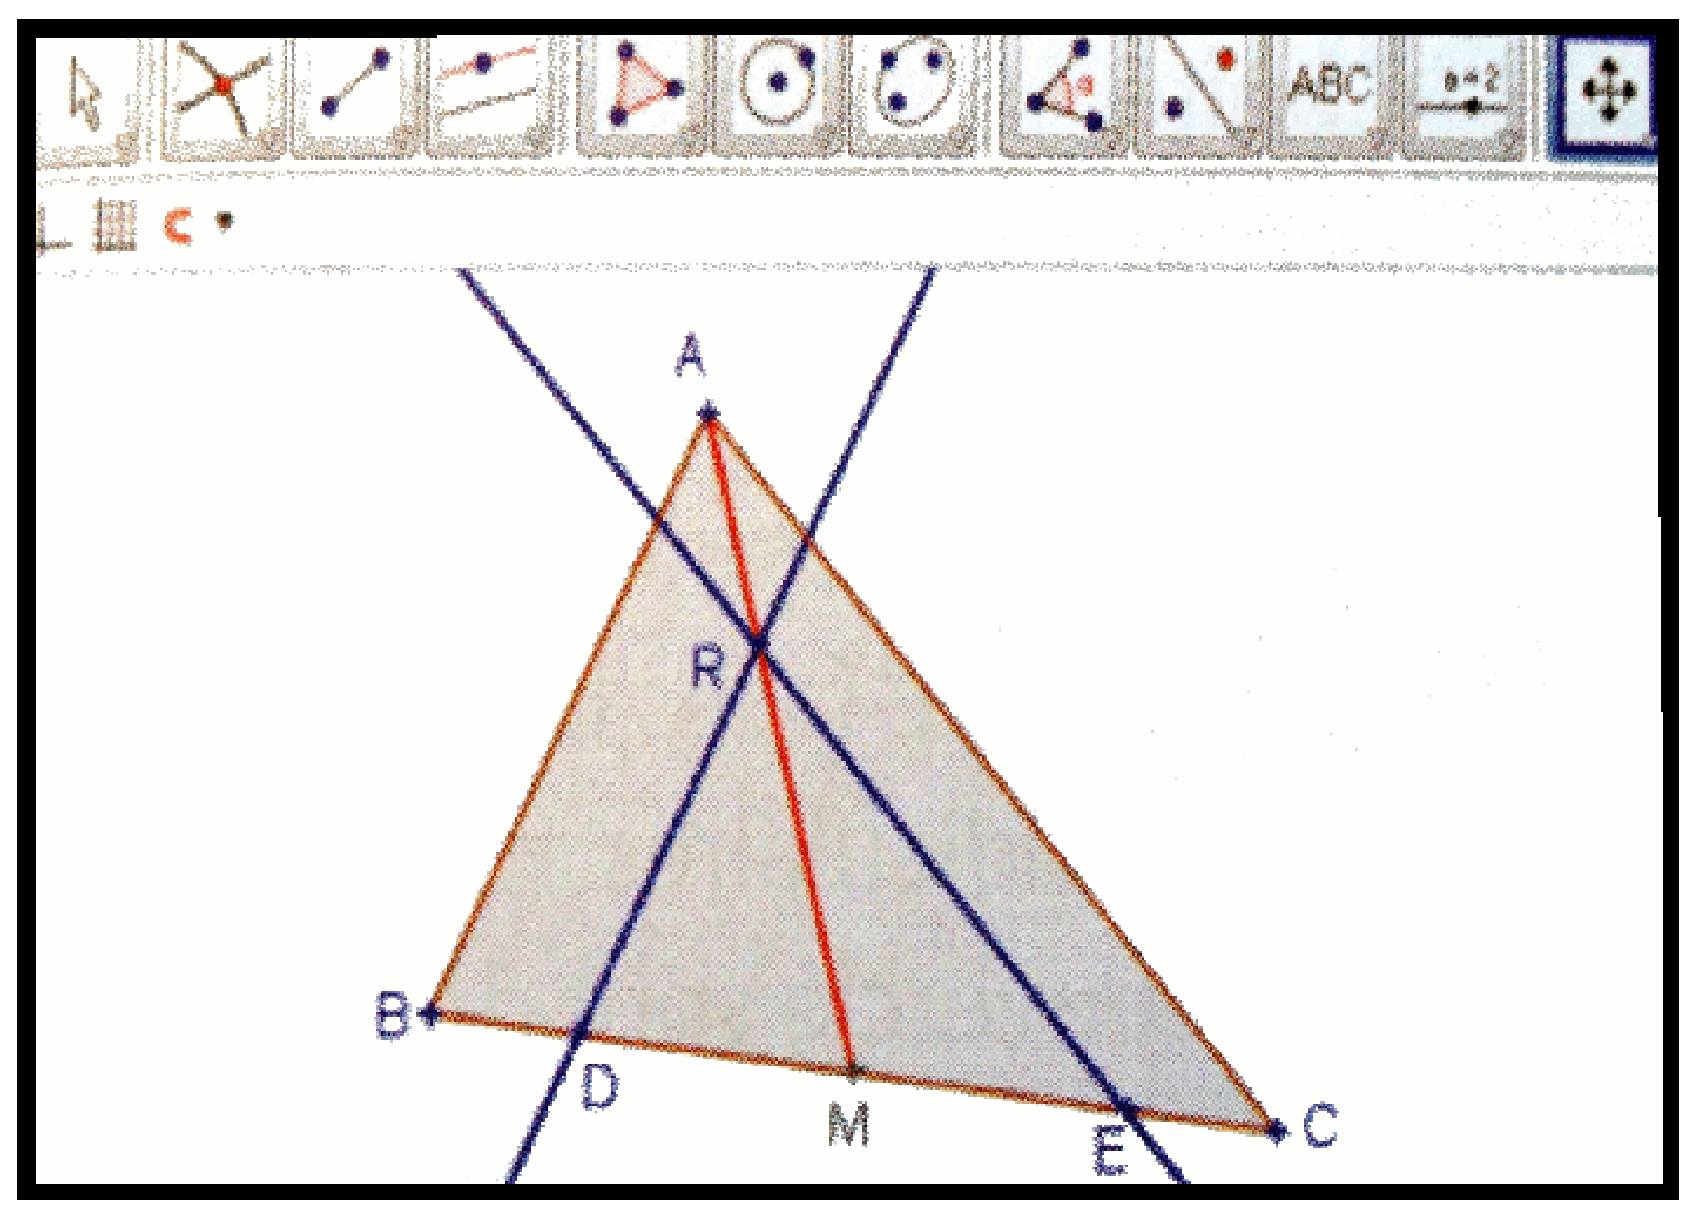
\includegraphics[width=6cm]{Geometrie/Images/G11_ex_geogebra}
   \end{center}
\end{exercice}

\begin{corrige}
\ \\ [-5mm]
    \begin{enumerate}
      \item À faire sur tablette ou ordinateur.
      \item On peut conjecturer que {\blue $MD =ME$}.
      \item On applique le Théorème de Thalès dans les triangles $AMB$ et $AMC$.
      \begin{itemize}
         \item Dans le triangle $AMB$, les points $M, R, A$ et $M, D, B$ sont alignés dans cet ordre. \\ [1mm]
            Les droites $(AB)$ et $(RD)$ sont parallèles donc, d'après le théorème de Thalès : $\dfrac{MR}{MA} =\dfrac{MD}{MB}$. \smallskip
         \item Dans le triangle $AMC$, les points $M, R, A$ et $M, E, C$ sont alignés dans cet ordre. \\ [1mm]
            Les droites $(AC)$ et $(RE)$ sont parallèles donc, d'après le théorème de Thalès : $\dfrac{MR}{MA} =\dfrac{ME}{MC}$. \smallskip
      \end{itemize}
      On a alors $\dfrac{MD}{MB} =\dfrac{ME}{MC}$. \\
      Or, $MB =MC$ puisque $M$ est le milieu de $[BC]$ d'où $\dfrac{MD}{MB} =\dfrac{ME}{MB} \iff$ {\blue MD = ME}.
   \end{enumerate}
\end{corrige}

\bigskip


\begin{exercice}[Puzzle de Lewis Carroll] %%%3
   On considère le carré de 8 carreaux de côté ci-dessous. En utilisant les triangles rectangles et les trapèzes rectangles constituant le carré comme des pièces de puzzle, on transforme ce carré en un rectangle de 5 carreaux sur 13 carreaux. Quel est le paradoxe considéré ici ? Démontez ce paradoxe.
   \begin{center}
   {\psset{unit=0.5}
      \begin{pspicture}(0,0)(8,8)
         \pspolygon[fillstyle=solid,fillcolor=FondTableaux,linewidth=0.8mm](0,0)(5,0)(5,3)(0,5)
         \pspolygon[fillstyle=solid,fillcolor=G1,linewidth=0.8mm](0,8)(5,8)(5,3)(0,5)
         \pspolygon[fillstyle=solid,fillcolor=B2,linewidth=0.1mm](5,0)(5,8)(8,8)
         \pspolygon[fillstyle=solid,fillcolor=BleuOuv,linewidth=0.1mm](5,0)(8,0)(8,8)
         \psgrid[subgriddiv=1,gridlabels=0](0,0)(8,8)
         \psframe[linewidth=0.8mm](5,0)(8,8)
         \psline[linewidth=0.8mm](5,0)(8,8)
      \end{pspicture}
      \qquad
      \begin{pspicture}(0,0)(13,8)
         \pspolygon[fillstyle=solid,fillcolor=FondTableaux,linewidth=0.8mm](0,0)(5,0)(5,3)(0,5)
         \pspolygon[fillstyle=solid,fillcolor=G1,linewidth=0.8mm](13,0)(13,5)(8,5)(8,2)
         \pspolygon[fillstyle=solid,fillcolor=BleuOuv,linewidth=0.1mm](5,0)(13,0)(5,3)
         \pspolygon[fillstyle=solid,fillcolor=B2,linewidth=0.1mm](0,5)(8,5)(8,2)
         \psgrid[subgriddiv=1,gridlabels=0](0,0)(13,5)
         \psline[linewidth=0.8mm](13,0)(5,0)(5,3)
         \psline[linewidth=0.8mm](5,3)(13,0)
         \psline[linewidth=0.8mm](0,5)(8,5)(8,2)
         \psline[linewidth=0.8mm](0,5)(8,2)
      \end{pspicture}
   }
   \end{center}
\end{exercice}

\begin{corrige}
   {\bf Aire des figures :} l'aire du carré vaut $8\,u.l.\times8\,u.l. =64\,u.a.$ et l'aire du rectangle vaut $13\,u.l.\times5\,u.l. =65\,u.a.$ \\
      On a donc \og 64 = 65 \fg{} et on a \og gagné \fg{} un carré unité entre les deux configurations. \\
   {\bf Explication du paradoxe :} dans le deuxième puzzle, on se place au niveau du trapèze gris et du triangle bleu que l'on schématise.
      \begin{center}
      {\psset{unit=0.5}
      \small
         \begin{pspicture}(0,-1)(13,4.5)
            \psgrid[subgriddiv=1,gridlabels=0](0,0)(13,5)
            \pspolygon[linewidth=0.8mm,linecolor=B1](0,0)(5,0)(5,3)(0,5)
            \psline[linewidth=0.8mm,linecolor=B1](5,0)(13,0)(5,3)
            \rput(-0.5,-0.5){$C$}
            \rput(5,-0.5){$B$}
            \rput(13.5,0){$A$}
            \rput(-0.5,5){$E$}
            \rput(5.5,3.5){$D$}
         \end{pspicture}
      }
      \end{center}
      On a : $\dfrac{AB}{AC} =\dfrac8{13}$ et $\dfrac{BD}{CE} =\dfrac35$. Or, $\dfrac8{13}\neq\dfrac35$, donc, l'une des hypothèses du théorème de Thalès n'est pas vérifiée.
      \medskip
      \begin{itemize}
         \item Les droites $(CE)$ et $(BD)$ sont parallèles puisque le quadrilatère $CBDE$ est un trapèze.
         \item Le triangle $DBA$ est rectangle en $B$ donc, $(BD) \perp (BA)$ et le quadrilatère $CBDE$ est rectangle en $B$ et $C$ donc, $(BD) \perp (BC)$, d'où $(BA)$ est parallèle à $(BC)$ et les points $A, B, C$ sont alignés dans cet ordre.
         \item Par conséquent, la seule condition non vérifiée est que les points $A, D, E$ ne sont pas alignés, et le carré unité supplémentaire se situe \og autour \fg{} de la diagonale $AE$.
      \end{itemize}
      {\bf Visuel :} si on affine le contour des figures, on \og voit \fg{} bien où se situe le problème.
      \begin{center}
      {\psset{unit=0.9}
         \begin{pspicture}(0,0)(13,5)
            \pspolygon[fillstyle=solid,fillcolor=FondTableaux,linewidth=0.1mm](0,0)(5,0)(5,3)(0,5)
            \pspolygon[fillstyle=solid,fillcolor=G1,linewidth=0.1mm](13,0)(13,5)(8,5)(8,2)
            \pspolygon[fillstyle=solid,fillcolor=BleuOuv,linewidth=0.1mm](5,0)(13,0)(5,3)
            \pspolygon[fillstyle=solid,fillcolor=B2,linewidth=0.1mm](0,5)(8,5)(8,2)
            \psgrid[subgriddiv=1,gridlabels=0](0,0)(13,5)
         \end{pspicture}
      }
      \end{center}
\end{corrige}

\bigskip


\begin{exercice}[Aire et volume] %%%4
   On considère la pyramide de sommet $S$ et de base $ABCD$ représentée ci-dessous. Les points $I, J, K$ et $L$ sont respectivement les milieux des arêtes $[SA], [SB], [SC]$ et $[SD]$. \\
   Parmi les affirmations suivantes, indiquer celle(s) qui est (sont) exacte(s) en justifiant. \\
   \begin{minipage}{6.5cm}
   {\psset{unit=0.8}
      \begin{pspicture}(-1,-0.4)(5,6)
         \psline(4,0)(0,0)
         \psline[linestyle=dashed](0,0)(2,2)(6,2)
         \psline(0,0)(3,5)(4,0)(6,2)(3,5)
         \psline[linestyle=dashed](1.5,2.5)(2.5,3.5)(4.5,3.5)
         \psline[linestyle=dashed](2,2)(3,5)
         \psline(1.5,2.5)(3.5,2.5)(4.5,3.5)
         \rput[bl](0,-0.4){$A$}
         \rput[bl](4.1,-0.3){$B$}
         \rput[bl](6.1,1.8){$C$}
         \rput[bl](2.0,1.6){$D$}
         \rput[bl](3,5.3){$S$}
        \rput[bl](2.6,3.2){$L$}
         \rput[bl](4.3,3){$K$}
         \rput[bl](3.7,2.3){$J$}
         \rput[bl](1.5,2.1){$I$}
      \end{pspicture}
   }
   \end{minipage}
   \begin{minipage}{10cm}
      \begin{enumerate}
         \item L'aire du quadrilatère $ABCD$ est égale à quatre fois l'aire du quadrilatère $IJKL$. 
         \item L'aire du quadrilatère $IJBA$ est égale à deux tiers de l'aire du triangle $SAB$.
         \item Le volume de la pyramide $SABCD$ est égal à trois fois celui de la pyramide $SIJKL$.
         \item Le volume de la pyramide $SABCD$ est égal aux huit septièmes du volume du solide $ABCDIJKL$. 
      \end{enumerate}
  \end{minipage}
\end{exercice}

\begin{corrige}
   {\bf Remarque de départ :} les points $I, J, K, L$ sont les milieux respectifs des arêtes $[SA], [SB], [SC], [SD]$. \\
   Donc, d'après le théorème de la droite des milieux appliqué aux triangles $SAB, SBC, SCD$ et $SDA$, on a $IJ =\dfrac12 AB, JK =\dfrac12 BC, KL =\dfrac12 CD, LI =\dfrac12DA$ et de plus, $IJ // AB, JK // BC, KL // CD$ et $LI // DA$. \\ [1mm]
   \begin{enumerate}
      \item D'après la remarque, le quadrilatère $ABCD$ est un  agrandissement du carré $IJKL$ de rapport 2, l'aire est donc multipliée par $2\times2 =4$. {\blue L'affirmation est vraie}.
      \item Le triangle $SAB$ est un agrandissement de coefficient $2$ du triangle $SIJ$. \\
         On a alors : $\mathcal{A}(SAB) =4\times \mathcal{A}(SIJ)$. \\
         Or, $\mathcal{A}(IJBA) =\mathcal{A}(SAB)-\mathcal{A}(SIJ) =\mathcal{A}(SAB)-\dfrac14\mathcal{A}(SAB) =\dfrac34\mathcal{A}(SAB)$.{\blue L'affirmation est fausse}.
      \item La pyramide $SABCD$ est un agrandissement de coefficient $2$ de la pyramide $SIJKL$ donc : \\
         $\mathcal{V}(SABCD) =2^3\times \mathcal{V}(SIJKL) =8\times\mathcal{V}(SIJKL)$. {\blue L'affirmation est fausse}.
      \item $\mathcal{V}(ABCDIJKL) =\mathcal{V}(SABCD)-\mathcal{V}(SIJKL) =\mathcal{V}(SABCD)-\dfrac18\mathcal{V}(SABCD) =\dfrac78\mathcal{V}(SABCD)$. \\
         Soit $\mathcal{V}(SABCD) =\dfrac87\mathcal{V}(SABCD)$. {\blue L'affirmation est vraie}.
   \end{enumerate}
\end{corrige}

\bigskip


\begin{exercice}[CRPE 2005 Créteil] %%%5
   Une station de sports d'hiver est équipée d'un téléphérique pour permettre aux skieurs d'atteindre un plateau en altitude. Des pylônes sont placés en A, E, C et B pour soutenir le câble que l'on considérera rectiligne. Le câble mesure \ukm{2,48}. L'altitude au point A est \um{2100}, l'altitude au point B est \um{2620}.
   \begin{enumerate}
      \item On définit la pente comme étant le rapport entre la hauteur du dénivelé (BB' sur le dessin) et la distance parcourue à l'horizontale (AB' sur le dessin). Calculer la pente de ce câble et l'exprimer en pourcentage.
      \item Entre B et C, le câble mesure 480 m.
      \begin{enumerate}
         \item Démontrer que CC' = \um{419} à \um{1} près.
         \item Calculer l'altitude au point C, arrondie à \um{1} près.
      \end{enumerate}
      \item
      \begin{enumerate}
         \item E est le milieu du segment [AC]. Calculer EC.
         \item Entre E et C, la cabine progresse à la vitesse constante de 5 m/s. En combien de temps la cabine parcourt-elle la distance EC ? Vous donnerez le résultat en minutes et secondes.
      \end{enumerate}
   \end{enumerate}
   \begin{center}     
   {\psset{unit=0.8}
   \footnotesize
      \begin{pspicture}(0,-0.5)(9,5)
        \pspolygon[linestyle=dotted](0,0)(9,0)
        \psline(0,0)(9,4)
        \psline[linestyle=dashed](9,0)(9,4)
        \psline[linestyle=dashed](3,0)(3,1.3)
        \psline[linestyle=dashed](6.5,0)(6.5,2.9)
        \psframe[fillstyle=solid,fillcolor=black](3,0)(3.2,0.2)
        \psframe[fillstyle=solid,fillcolor=black](6.5,0)(6.7,0.2)
        \psframe[fillstyle=solid,fillcolor=black](9,0)(9.2,0.2)
       \psline(4.5,2)(4.5,1.7)
        \pswedge[fillstyle=solid,fillcolor=black](0,0){0.8}{0}{24}
        \psframe[fillstyle=solid,fillcolor=black](4.2,1.4)(4.8,1.7)
        \rput(0,-0.5){départ}
        \rput(9.7,4){arrivée}
        \rput(4.8,-0.5){ligne horizontale}
        \rput(0,0.5){pylône 1}
        \rput(3,2){pylône 2}
        \rput(6.5,3.6){pylône 3}
        \rput(9,4.7){pylône 4}
        \rput(4.5,1.2){cabine}
        \rput(-0.3,0){A}
        \rput(3,-0.3){E'}
        \rput(6.5,-0.3){C'}
        \rput(9,-0.3){B'}
        \rput(3,1.6){E}
        \rput(6.5,3.2){C}
        \rput(9,4.3){B}
        \rput(1.1,0.25){$\alpha$}
     \end{pspicture}
   }
   \end{center}     
   {\it Remarque : sur ce schéma, les mesures des longueurs et de l'angle ne sont pas respectées.}
\end{exercice}

\begin{corrige}
\ \\ [-5mm]
   \begin{enumerate}
      \item Pour déterminer la pente $p$ du câble égale à $\dfrac{\text{BB'}}{\text{AB}}$, on peut utiliser par exemple des formules de \\ [1mm]
         trigonométrie : $\sin(\alpha) =\dfrac{\text{BB'}}{\text{AB}} =\dfrac{\um{2620}-\um{2100}}{\um{2480}} =\dfrac{\um{520}}{\um{2480}} \iff \alpha =\arcsin\left(\dfrac{520}{2\,480}\right) \approx\udeg{12,10}$. \\ [1mm]
         La pente est donc égale à $\dfrac{\text{BB'}}{\text{AB'}} =\tan(\widehat{\alpha}) =\tan(\udeg{12,10}) \approx0,2144$. \\ [1mm]
         {\blue La pente du câble est de 21,44\,\% environ}.
      \item 
      \begin{enumerate}
         \item Dans la triangle ACC' rectangle en C', on a : $\sin(\alpha) =\dfrac{\text{CC'}}{\text{AC}} \iff \sin(\udeg{12,10}) =\dfrac{\text{CC'}}{\um{2000}}$ \\ [1mm]
         $\iff \text{CC'} =\um{2000}\times\sin(\udeg{12,10}) \approx\um{419,24}$. \\
         {\blue La longueur du segment [CC'] est de 419 mètres environ}.
         \item Le point C' est à l'altitude de départ, c'est-à-dire \um{2100}. Or, \um{2100} + \um{419} = \um{2519} ; donc, \\
         {\blue le point C est à une altitude de \um{2519} environ.}
      \end{enumerate}
      \setcounter{enumi}{2}
      \item
      \begin{enumerate}
         \item On a AC $=\um{2480}-\um{480} =\um{2000}$ et E est le milieu de [AC], donc EC $=\um{2\,000}\div2 =\um{1000}$. \\
         {\blue EC = 1000 m.}
         \item Soit $t$ le temps mis par la cabine pour aller de E à C, on utilise la formule : \\ [1mm]
         $v =\dfrac{d}{t} \iff \ums{5} =\dfrac{\um{1000}}{t}$ \\
         \hspace*{0.9cm} $\iff t = \dfrac{\um{1000}}{\ums{5}}$ \\ [1.5mm]
         \hspace*{0.9cm} $\iff t  =\us{200}$. \\
         Or, $\us{200} =\us{180}+\us{20}$, donc, \\ 
         {\blue il faudra 3 minutes et 20 secondes à la cabine pour parcourir la distance EC}.
      \end{enumerate}
   \end{enumerate}
\end{corrige}

\bigskip


\begin{exercice}[CRPE 2018 G1] %%%6
   \begin{minipage}{7.5cm}
      Un éleveur possède un silo à farine formé de deux solides de révolution : un cône et un cylindre, comme représenté sur la figure ci-contre. \\
      Ces deux solides ont le même axe de révolution. Les centres D et A des bases sont alignés avec le sommet S du cône. \\
      On donne : AS = \um{1,60} ; DA = \um{2,40} ; AB = \um{1,30}. \\ [5mm]
      {\it Cette figure n'est pas à l'échelle.}
   \end{minipage}
   \begin{minipage}{7cm}
   {\psset{unit=0.65}
   \small
      \begin{pspicture}(-4,-1.5)(7,7)
         \psframe[linecolor=gray,fillstyle=solid,fillcolor=gray](1.5,0)(1.75,0.25)
         \psframe[linecolor=gray,fillstyle=solid,fillcolor=gray](3,0)(3.25,0.25)
         \psline(0,7)(0,2)(1.5,0)(3,2)
         \psellipse(1.5,7)(1.5,0.18)
         \psellipse[linestyle=dashed,linewidth=0.1mm](1.5,2)(1.5,0.18) 
         \pscurve(0,2)(0.5,1.88)(0.75,1.85)(1.5,1.825)(2.25,1.85)(2.5,1.88)(3,2)
         \psline(3,0)(3,7)(1.5,7)
         \psline(-1,0)(7.5,0)
         \psline(3,7)(7,0)
         \psline(3,2)(4.3,0)
         \psline[linestyle=dashed](1.5,0)(1.5,7)
         \psline[linestyle=dashed](1.5,2)(3,2)
         \rput(1.5,-0.3){S}
         \rput(3,-0.3){H}
         \rput(4.3,-0.3){M}
         \rput(7,-0.3){N}
         \rput(1.3,2){A}
         \rput(3.3,2){B}
         \rput(1.3,7){D}
         \rput(3.3,7){C}
      \end{pspicture}
   }
   \end{minipage}
   \begin{enumerate}
      \item Quel est le volume en mètre cube du silo à farine ? Arrondir au centième.
     \item Le silo est rempli de farine d’orge au $\dfrac67$ de son volume total. Une vache mange en moyenne 3 L de farine par jour. L’éleveur possède 48 vaches. Aura-t-il assez de farine pour nourrir ses 48 vaches durant 90 jours ?
      \item Pour réaliser des travaux, deux échelles ont été posées contre le silo. Elles sont représentées sur la figure par des segments [BM] et [CN]. \\
         On donne SM = \um{2,} et SN = \um{3,3}. On note H le pied de la hauteur issue de B dans le triangle SBM. Les points S, H, M et N sont alignés. Les points C, B et H sont alignés. \\
         Les deux échelles sont-elles parallèles ? Justifier la réponse.
   \end{enumerate}
\end{exercice}

\begin{corrige}
\ \\ [-5mm]
   \begin{enumerate}
      \item Volume du cylindre en mètre cube : $V_{\text{cylindre}} = \pi\times1,3^2\times2,4$ ; \\ [1mm]
         Volume du cône en mètre cube : $V_{\text{cône}} = \dfrac13\times\pi\times1,3^2\times1,6$ ; \\
         Volume du silo en mètre cube : $V =V_{\text{cylindre}}+V_{\text{cône}} =4,056\pi+\dfrac13\times2,704\pi \approx 15,5739$. \\
         {\blue Le silo a un volume d'environ \umc{15,57}}.
      \item Quantité de farine en litre pour 48 vaches pendant 90 jours : $C_{\text{vaches}} =90\times48\times\ul{3} =\ul{12\,960}$. \\
         Capacité en litre du silo : $C_{\text{silo}} \approx\dfrac67\times\umc{15,5739} \approx\dfrac67\times\udmc{15573,9} \approx\dfrac67\times\ul{15573,9} \approx \ul{13349}$. \\
         On a $C_{\text{silo}}>C_{\text{vaches}}$ donc, {\blue l'éleveur aura suffisamment de farine pour nourrir ses 48 vaches pendant 90 jours}.
      \item Remarque : A et D  sont les centres des bases des solides de révolution, donc (SA) est orthogonale à la base du cône et (AD) est orthogonale à la base du cylindre. On a alors (SA) perpendiculaire à (AB) et (AD) perpendiculaire à (DC) et à (AB). \\
         D'où ABHS et ABCD sont des rectangles et leurs côtés sont deux à deux égaux et parallèles. \\
         Les points H, M, N et H, B, C sont alignés dans cet ordre. \\ [1mm]
         On calcule les rapports $\dfrac{\text{HN}}{\text{HM}}$ et $\dfrac{\text{HC}}{\text{HB}}$ avec les valeurs suivantes : \\ [1mm]
         HN = SN $-$ SH = SN $-$ AB = \um{3,3} $-$ \um{1,3} = \um{2}. \\
         HM = SM $-$ SH = SM $-$ AB = \um{2,1} $-$ \um{1,3} = \um{0,8}. \\
         HC = HB + BC = SA + AD = \um{1,6} + \um{2,4} = \um{4}. \\
         HB = SA = \um{1,6}. \\ [1mm]
         D'où $\dfrac{\text{HN}}{\text{HM}} =\dfrac{\um{2}}{\um{0,8}} =2,5$ et $\dfrac{\text{HC}}{\text{HB}} =\dfrac{\um{4}}{\um{1,6}} =2,5$. \\ [1mm]
         Les rapports sont égaux, donc d'après la réciproque du théorème de Thalès, les droites (NC) et (MB) sont parallèles. {\blue Les deux échelles sont parallèles}.
   \end{enumerate}
\end{corrige}

\bigskip


\begin{exercice}[CRPE 2015 G1] %%%7
   {\it Dans cet exercice, on prendra \ucm{1} comme unité de longueur.} \\ [5mm]
   On considère un trapèze $ABFE$ rectangle en $A$ et $B$, c'est-à-dire tel que les droites ($AE$) et ($BF$) sont perpendiculaires à la droite ($AB$), et tel que $AB = 14$ ; $AE = 3$ ; $BF = 9$. \\
   Le point $M$ est un point variable sur le segment [$AB$]. \\
   Le but de cet exercice est de déterminer la position de $M$ pour laquelle la valeur de $EM+MF$ est minimale.
   \begin{enumerate}
      \item Construire le trapèze $ABFE$ et le point $G$, symétrique du point $F$ par rapport à la droite ($AB$).
      \item On appelle $P$ l'intersection des droites ($AB$) et ($EG$). \\
   Montrer que pour tout point $M$ de [$AB$], on a : $EM+MG\geqslant EP+PG$. \\
         En déduire que la valeur $EM+MF$ est minimale lorsque $M$ est placé en $P$.
      \item Montrer que $\dfrac{AP}{14-AP} =\dfrac39$ puis calculer $AP$. \smallskip
      \item Calculer la valeur minimale de $EM+MF$. En donner la valeur exacte en cm, et arrondie au dixième.
   \end{enumerate}
\end{exercice}

\begin{corrige}
\ \\ [-5mm]
   \begin{enumerate}
      \item La figure suivante est à l'échelle 1\slash3. \\   
      \begin{pspicture}(-5,-3.5)(5,2.5)
      {\psset{unit=0.33}
         \pstGeonode[PosAngle={180,0,0,180,0,45,45}]{A}(14,0){B}(14,9){F}(0,3){E}(14,-9){G}(3.5,0){P}(8,0){M}
         \pstLineAB{A}{B}
         \pstLineAB{B}{F}
         \pstLineAB{F}{E}
         \pstLineAB{E}{A}      
         \pstLineAB[linewidth=0.5mm,linecolor=B1]{E}{G}
         \pstLineAB[linestyle=dashed,linecolor=A1]{E}{M}
        \pstLineAB[linestyle=dashed,linecolor=A1]{M}{G}
         \pstRightAngle[linecolor=G1]{E}{A}{B}
         \pstRightAngle[linecolor=G1]{A}{B}{F}  
         \pstSegmentMark{B}{F}
         \pstSegmentMark{B}{G}}   
      \end{pspicture}
      \item Le point $P$ est situé sur le segment [$EG$], par construction. On a donc $EP+PG =EG$. \\
         Tout point $M$ du plan non situé sur le segment [$EG$] vérifie \\
         $EM+MG > EG$, soit $EM+MG > EP+PG$. \\
         Si le point $M$ appartient au segment [$EG$], on a $EM+MG = EP+PG$. \\
         Pour tout point $M$ de [$AB$], on a {\blue $EM+MG \geqslant EP+PG$ avec égalité lorsque $M$ est placé en $P$.} \\
         $G$ est le symétrique de $F$ par rapport à $B$ donc, $B$ est le milieu du segment [$FG$]. \\
         La droite ($AB$) est perpendiculaire à la droite ($FB$). Donc, ($AB$) est la médiatrice du segment [$FG$]. \\
         Le point $M$ étant situé sur la médiatrice de [$FG$], il est à égale distance des points $F$ et $G$, c'est-à-dire $MF =MG$ et on a alors $EM+MG = EM+MF$. \\
         La valeur minimale de $EM+MF$ correspond donc à la valeur minimale de $EM+MG$, qui est $EP+PG$. \\
         {\blue La valeur $EM+MF$ est minimale lorsque $M$ est placé en $P$}.  
      \item Les droites ($EA$) et ($FB$) sont toutes deux perpendiculaires à la même droite ($AB$), elles sont donc parallèles entre elles. \\
         Les points $F, B$ et $G$ sont alignés donc, les droites ($EA$) et ($BG$) sont parallèles. \\ 
         Les points $E, P, G$ et $A, P, B$ sont alignés dans le même ordre. \\
         On peut donc appliquer le théorème de Thalès et sa conséquence : $\dfrac{PE}{PG} =\dfrac{PA}{PB}  =\dfrac{EA}{GB}$. \\
         Or, $P\in[AB]$ donc $AP+PB =AB \iff PB =14-AP$. \\
         Avec $EA =3$ et $GB =FB =9$, on obtient bien \quad {\blue $\dfrac{AP}{14-AP} =\dfrac{3}{9}$.}
         $\dfrac{AP}{14-AP} =\dfrac{3}{9} \iff 9\times AP =3\times(14-AP) \iff 9AP+3AP =42 \iff AP =\dfrac{42}{12} =\dfrac{7}{2}.$ \\ [1mm]
         {\blue La mesure de $AP$ est de \ucm{3,5}}.
      \item D'après le question 2), la valeur minimale de $EM+MF$ est atteinte lorsque $M$ est en $P$. Calculons $EP+PF$.
         \begin{itemize}
            \item Calcul de $EP$. Dans le triangle $EAP$ rectangle en $A$, d'après le théorème de Pythagore : \\
               $EP^2 = EA^2 + AP^2=3^2+\left(\dfrac72\right)^2=9+\dfrac{49}{4}=\dfrac{85}{4}$, \quad soit $EP =\dfrac{\sqrt{85}}{2}$.
            \item Calcul de $PF$. Dans le triangle $PBF$ rectangle en $B$, d'après le théorème de Pythagore : \\
               $PF^2 =PB^2+BF^2$ avec $PB =AB-AP =14-\dfrac72 =\dfrac{21}{2}$. \\
               D'où  $PF^2=\left(\dfrac{21}{2}\right)^2+9^2 =\dfrac{441}{4}+81=\dfrac{765}{4}$, \quad soit $PF=\dfrac{3\sqrt{85}}{2}$. \\
         \end{itemize}
         Pas conséquent, $EP+PF =\dfrac{\sqrt{85}}{2}$ + $\dfrac{3\sqrt{85}}{2} =2\sqrt{85}\approx 18,44$. \\
         {\blue La valeur minimale de $EM+MF$ est de $2\sqrt{85} \ucm{}\approx \ucm{18,4}$}.
   \end{enumerate}
\end{corrige}

\bigskip


\begin{exercice}[CRPE 2008 Paris]
   On considère trois cercles $(C_1), (C_2)$ et $(C_3)$ de même rayon, noté $r$, et de centres respectifs $I, O$ et $J.$ Dans tout l'exercice, le rayon $r$ est un nombre entier non nul. Nous savons que :
   \begin{itemize}
      \item les trois points $I, O $ et $J$ sont alignés et dans cet ordre ;
      \item le cercle $(C_1)$ est tangent au cercle $(C_2)$, le cercle $(C_2)$ est tangent au cercle $(C_3)$ ;
      \item le point $E$ est à l'intersection de la droite $(OI)$ et du cercle $(C_1)$, et n'appartient pas au cercle $(C_2)$ ;
      \item la droite $(\Delta)$ est tangente au cercle $(C_3)$ en $T$ et passe par $E$ ; elle coupe le cercle $(C_2)$ en $A$ et en $B$ ;
      \item $H$ est le point de $(\Delta)$ tel que $(OH)$ et $(\Delta)$ sont perpendiculaires.
   \end{itemize}
   {\psset{algebraic=true,unit=0.9}
      \begin{pspicture}(-6,-2.5)(11,3.5)
         \pspolygon(7.18,1.87)(7.27,1.46)(7.68,1.54)(7.6,1.96)
         \psline(3.5,1.1)(3.55,0.8)(3.8,0.85)
         \psplot{-3.}{11.}{(-0.-0.*x)/4.}
         \pscircle(0,0){2}
         \pscircle(4,0){2}
         \pscircle(8,0){2}
         \psplot{-3}{11}{(--3.92--1.96*x)/9.6}
         \psline(7.6,1.96)(8,0)
         \psline(3.76,1.18)(4,0)
         \psdots(0,0)(4,0)(8,0)(-2,0)(7.6,1.96)(2.19,0.86)(5.33,1.5)(3.76,1.18)
         \rput[bl](-0.1,-0.6){$I$}
         \rput[bl](3.9,-0.6){$O$}
         \rput[bl](7.9,-0.6){$J$}
         \rput[bl](-2.4,0.2){$E$}
         \rput[bl](7.5,2.2){$T$}
         \rput[bl](1.9,1.1){$A$}
         \rput[bl](5.4,1.7){$B$}
         \rput[bl](3.7,1.4){$H$}
         \rput(10,2){$(\Delta)$}
      \end{pspicture}}

   {\bf On pose $OH = a$}
   \begin{enumerate}
      \item En utilisant le théorème de Thalès, démontrer que : $a =\dfrac35r$.
      \item Expliquer pourquoi le nombre $a$ est toujours un nombre rationnel.
      \item $a$ est-il toujours un nombre décimal ? Justifier la réponse.
      \item Quels sont les nombres $r$ pour lesquels $a$ est un nombre entier ?
      \item Le nombre $a$ peut-il être un nombre premier ?
      \item Calculer $HB$ en fonction de $r$. \\ [5pt]
      \hspace*{-0.5cm} {\bf On pose $AB = b$}
      \item Démontrer que $H$ est le milieu de $[AB]$ et en déduire que $b =\dfrac85r$. \smallskip
      \item Existe-t-il des nombres $r$ pour lesquels le nombre $b$ est un nombre premier ? Justifier.
   \end{enumerate}
\end{exercice}

\begin{corrige}
\ \\ [-5mm]
   \begin{enumerate}
      \item D'après l'énoncé, les droites $(OH)$ et $(\Delta)$ sont perpendiculaires. \\
         Par ailleurs, la droite $(\Delta)$ est tangente en $T$ à $(C_3)$, donc les droites $(JT)$ et ($\Delta)$ sont perpendiculaires. \\
         Par conséquent, les droites $(OH)$ et $(JT)$ sont parallèles comme droites perpendiculaires à la même droite $(\Delta)$. \\
         De plus, les points $E, H$ et $T$ sont alignés dans cet ordre et les points $E, O $ et $J$ sont alignés dans cet ordre. \\
         D'après le théorème de Thalès : $\dfrac{EO}{EJ} =\dfrac{EH}{ET} =\dfrac{OH}{JT}$ \\ [1mm]
         \hspace*{4.2cm} $\Rightarrow \dfrac{3r}{5r} =\dfrac{a}{r}$ \\ [1mm]
         \hspace*{4.3cm} $\Rightarrow a =\dfrac{3r^2}{5r} =\dfrac{3r}{5}$. \quad D'où on a bien {\blue $a =\dfrac35r$.}
      \item $a$ s'écrit sous la forme $\dfrac{p}{q}$ avec $p =3r$ ($r$ entier) et $q =5$ (entier). \\ [1mm]
         Pas définition, {\blue $a$ est un nombre rationnel comme quotient de deux entiers}.
      \item $a =\dfrac35r =\dfrac{6r}{10}$ avec $6r$ un nombre entier, donc $a$ peut s'écrire sous la forme d'une fraction décimale. \\ [1mm]
         D'où : {\blue $a$ est toujours un nombre décimal}.
      \item $a =\dfrac{3r}{5}$ donc, $a$ est un nombre entier si, et seulement si, $3r$ est divisible par 5. \\ [1mm]
         Or, 3 et 5 sont premiers entre eux, donc $r$ doit être divisible par 5 ce qui signifie qu'il est multiple de 5. \\
         {\blue $a$ est un nombre entier si, et seulement si, $r$ est  multiple de 5}.
      \item Pour que $a$ soit un nombre premier, il faut que $a$ soit un nombre entier et qu'il soit divisible uniquement par 1 et lui-même. Or $a$ est entier si et seulement si $r$ est multiple de 5 d'après la question précédente, c'est-à-dire s'il s'écrit $r = 5k$, où $k$ est un entier. \\
         Dans ce cas, $a = \dfrac{3\times\cancel{5}k}{\cancel{5}} =3k$. \\ [1mm]
         $a$ est donc un multiple de $3$. Il ne peut être premier que lorsque $k$ est égal à 1, c'est-à-dire $r = 5\times1 =5$. \\
         {\blue $a$ ne peut être premier que s'il prend la valeur 3}. \footnote{La question demande seulement si le nombre $a$ peut être un nombre premier, donc une réponse du type \og Pour $r =5$ on obtient $a =3$ qui est bien un nombre premier \fg{} est tout à fait juste.}
      \item On applique le théorème de Pythagore dans le triangle rectangle $OHB$ rectangle en $H$ : \\
         $OB^2 = OH^2+ HB^2 \iff HB^2 = OB^2-OH^2$ \\
         \hspace*{4.4cm} $=r^2-\left(\dfrac35r\right)^2$ \\ [1mm]
         \hspace*{4.4cm} $= \dfrac{25}{25}r^2-\dfrac{9}{25}r^2$ \\ [1mm]
         \hspace*{4.4cm} $= \dfrac{16}{25} r^2$. \qquad D'où : {\blue $HB =\dfrac45r$.}
         \smallskip
      \item Dans le triangle $OAB$, on a $OA = OB$ donc, $O$ appartient à la médiatrice du segment $[AB]$. \\
         De plus, la droite $(OH)$ est perpendiculaire à la droite $(AB)$, donc la droite $(OH)$ est la médiatrice du segment $[AB]$ : elle coupe $[AB]$ en $H$, on milieu. \\
         $H$ étant le milieu du segment $[AB]$, on a $b =AB = 2HB =2\times\dfrac45r =\dfrac{8}{5}r$. \\
         D'où : {\blue Le point $H$ est le milieu de $[AB]$ et on a $b =\dfrac{8}{5}r$.}
         \smallskip
      \item Pour que $b$ soit un nombre premier, il faut que $b$ soit un nombre entier et qu'il soit divisible uniquement par 1 et lui-même. Or $b$ est entier si et seulement si $8r$ est est divisible par 5. Avec 8 et 5 premiers entre eux, c'est dont $r$ qui doit être divisible par 5, c'est-à-dire qu'il s'écrit $r = 5k$, où $k$ est un entier. \\
         Dans ce cas, $b =\dfrac{8\times\cancel{5}k}{\cancel{5}} =8k$. \\
         $b$ est alors un multiple de 8 et comme $8 =2^3$ est composé, $b$ ne peut jamais être un nombre premier. \\
         {\blue Il n'existe pas de nombre $r$ tel que $b$ soit premier.}
   \end{enumerate}
\end{corrige}

\bigskip


\begin{exercice}[CRPE 2016 G2]
   Cet exercice porte sur l'utilisation d'un appareil photo numérique et étudie son fonctionnement. \\
   \begin{minipage}{9cm}
      {\bf L'appareil photo : notations et vocabulaire.} \\ [5mm]
      \begin{itemize}
         \item $L$ est la largeur de la scène photographiée ;
         \item $\alpha$ est l'angle de champ (angle sous lequel la scène est vue) ;
         \item $\ell$ est la largeur du capteur numérique situé à l'arrière de l'appareil photo ;
         \item $D$ est la distance entre la scène photographiée et le capteur numérique ;
         \item $f$, qui sera appelée focale de l'objectif, est la distance entre le capteur et le centre optique de l'objectif. C'est une caractéristique essentielle d'un objectif. Elle s'exprime généralement en millimètre (mm).
      \end{itemize}
   \end{minipage}
   \hspace{2cm}
   \begin{minipage}{5cm}
      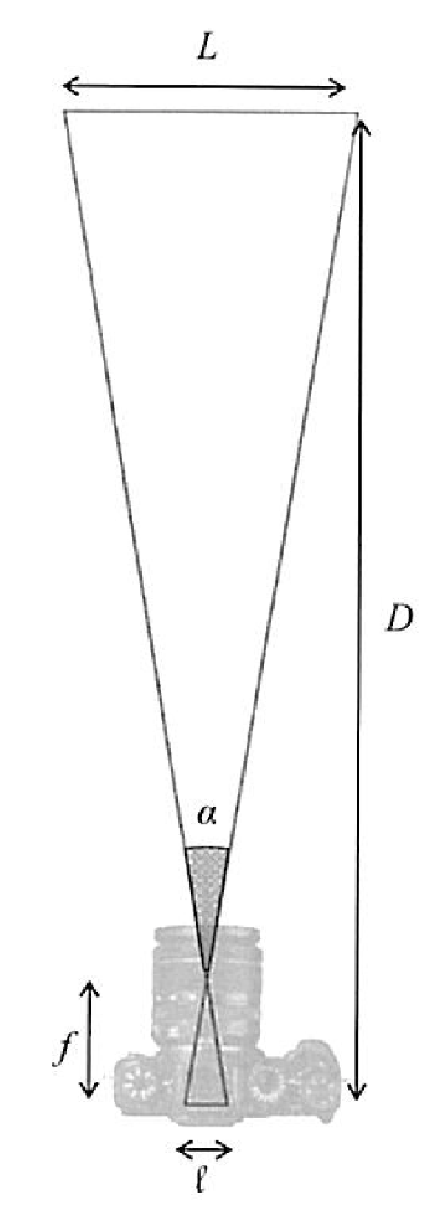
\includegraphics[width=3.5cm]{Geometrie/Images/G11_ex_appareil_photo}
   \end{minipage}

   \bigskip
   On schématise la situation par la figure ci-dessous dans laquelle les droites $(AA'), (BB')$ et $(HK)$ sont concourantes en $C$. \\
   \begin{minipage}{7.5cm}
      \begin{pspicture}(-0.5,-2)(7,8)
         \pspolygon(0,6)(4,6)(1,0)(3,0)
         \psframe(2,6)(2.2,5.8)
         \psframe(2,0)(1.8,0.2)
         \psline{<->}(4.5,2)(4.5,0)
         \rput(4.8,1){$f$}
         \psline{<->}(5.5,6)(5.5,0)
         \rput(5.8,3){$D$}
         \psline{<->}(0,7)(4,7)
         \rput(2,7.3){$L$}
         \psline[linestyle=dashed](2,0)(2,6)
         \psline{<->}(1,-1)(3,-1)
         \rput(2,-1.3){$\ell$}
         \psline[linestyle=dotted](3.5,0)(5.5,0)
         \psline[linestyle=dotted](2.5,2)(4.5,2)
         \psline[linestyle=dotted](4.5,6)(5.5,6)
         \psline[linestyle=dotted](0,6.5)(0,7)
         \psline[linestyle=dotted](4,6.5)(4,7)
         \psline[linestyle=dotted](1,-0.5)(1,-1)
         \psline[linestyle=dotted](3,-0.5)(3,-1)
         \psarc(2,2){0.75}{62}{118}
         \rput(2.25,3){$\alpha$}
         \rput(1,6){/\!\!/}
         \rput(3,6){/\!\!/}
         \rput(1.5,0){x}
         \rput(2.5,0){x}
         \begin{small}
            \rput(-0.3,6.3){$A$}
            \rput(4.3,6.3){$B$}
            \rput(0.7,-0.3){$B'$}
            \rput(3.3,-0.3){$A'$}
            \rput(2,-0.3){$K$}
            \rput(2,6.3){$H$}
            \rput(1.5,2){$C$}
         \end{small}
      \end{pspicture}
   \end{minipage}
   \begin{minipage}{9.5cm}
      \begin{enumerate}
         \item À l'aide des informations portées sur la figure :
            \begin{enumerate}
               \item Justifier que les droites $(AH)$ et $(A'K)$ sont parallèles.
               \item Démontrer que la droite $(HK)$ est un axe de symétrie de la figure.
            \end{enumerate}
         \item Justifier l'égalité : $\dfrac{CH}{CK} =\dfrac{AH}{A'K}$. \smallskip
         \item En déduire la relation : $\dfrac{D}{f} =\dfrac{L}{\ell}+1$.
         \item On considère que le capteur de l'appareil a pour largeur $\ell =\umm{36}$ et que le photographe est placé à $D =\um{12}$ de la scène du théâtre au centre de la salle.
         \begin{enumerate}
            \item Déterminer la largeur de la scène photographiée $L$ qui correspond à une focale de \umm{35}.
            \item La scène du théâtre mesure \um{15} de large. Quelles focales, en millimètre, le photographe peut-il utiliser pour que la largeur de la scène photographiée soit au moins aussi grande que la largeur de la scène du théâtre ?
         \end{enumerate}
      \end{enumerate}
   \end{minipage}
\end{exercice}

\begin{corrige}
\ \\ [-5mm]
   \begin{enumerate}
      \item
         \begin{enumerate}
            \item Les droites $(AH)$ et $(A'K)$ sont toutes deux perpendiculaires à la même droite $(HK)$ donc, \\
               {\blue les droites $(AH)$ et $(A'K)$ sont parallèles}.
            \item La droite $[HK]$ passant par $C$ est la médiatrice des segments $[AB]$ et $[A'B']$ (droite perpendiculaire aux segments passant par leur milieu) donc, {\blue c'est un axe se symétrie de la figure}.
         \end{enumerate}
      \setcounter{enumi}{1}
      \item Les points $A, C, A'$ et $H, C, K$ sont alignés dans cet ordre et les droites $(AH)$ et $(A'K)$ sont parallèles, \\ [1mm]
         on peut donc appliquer le théorème de Thalès : $\dfrac{CH}{CK} =\dfrac{CA}{CA'} =\dfrac{HA}{KA'}$ soit \quad {\blue $\dfrac{CH}{CK} =\dfrac{HA}{A'K}$}. \\
      \item $\dfrac{CH}{CK} =\dfrac{HA}{A'K} \iff \dfrac{D-f}{f} =\dfrac{\dfrac{L}{2}}{\dfrac{\ell}{2}} \iff \dfrac{D}{f}-\dfrac{f}{f}=\dfrac{L}{\cancel{2}}\times\dfrac{\cancel{2}}{\ell} \iff$ {\blue $\dfrac{D}{f} =\dfrac{L}{\ell}+1$}. \\ [1mm]
      \item
         \begin{enumerate}
            \item On a $\ell =\umm{36}$ ; $D =\um{12} =\umm{12000}$ et $f =\umm{35}$ soit, avec des mesures en millimètre : \\ [1mm]
               $\dfrac{12\,000}{35} =\dfrac{L}{36}+1 \iff \dfrac{L}{36} =\dfrac{12\,000}{35}-1 \iff \dfrac{L}{36} =\dfrac{11\,965}{35} \iff L =\dfrac{11\,965\times36}{35} \approx 12\,306,9$. \\ [1mm]
               {\blue La scène photographiée mesure environ \um{12,3}}.
            \item On a $\ell =\umm{36}$ ; $D =\um{12} =\umm{12000}$ et $L =\um{15} =\umm{15000}$ soit, avec des mesures en millimètre : \\ [1mm]
               $\dfrac{12\,000}{f} =\dfrac{15\,000}{36}+1 \iff \dfrac{12\,000}{f}  =\dfrac{15\,036}{36} \iff f =\dfrac{12\,000\times36}{15\,036} \approx 28,7$. \\ [1mm]
               Avec une focale d'environ \umm{28,7}, la scène photographiée mesure environ mesure \um{15} de large. Or, lorsqu'on diminue la focale $f$, on augmente la largeur de la scène photographiée donc, \\
               {\blue il faut utiliser une focale inférieure ou égale à \umm{28,7} pour photographier une scène de \um{15} au moins}.
         \end{enumerate}
   \end{enumerate}
\end{corrige}

\bigskip


\begin{exercice}[CRPE 2019 G1] %%% 8
   La figure ci-dessous -- qui n’est pas nécessairement à l’échelle -- représente trois carrés dont les mesures des côtés, en centimètre, sont respectivement \ucm{3}, \ucm{4} et \ucm{5}. Les deux plus petits carrés sont gris, le troisième est blanc.
   \begin{center}
      {\psset{unit=0.47}
      \begin{pspicture}(0,0.5)(15,5)
         \psframe[fillstyle=solid,fillcolor=gray!60](0,0)(3,3)
         \psframe[fillstyle=solid,fillcolor=gray!60](3,0)(7,4)
         \psframe(7,0)(12,5)
      \end{pspicture}}
   \end{center}
   \begin{enumerate}
      \item Vérifier que la somme des aires des deux carrés gris est égale à l’aire du carré blanc.
      \item Claude affirme : \og Si on dispose les trois carrés obtenus à la question précédente comme sur la figure 1 ci-dessous, alors le triangle $ABC$ est un triangle rectangle. \fg. \\
         L’affirmation de Claude est-elle vraie ou fausse ? Justifier la réponse.
         \begin{center}
         {\psset{unit=0.47}
         \small
            \begin{pspicture}(-1,-1)(11,12.2)
               \psframe[fillstyle=solid,fillcolor=gray!60,CurveType=polygon](3,0)(7,4)
               \psframe[fillstyle=solid,fillcolor=gray!60](0,4)(3,7)
               \pspolygon(7,4)(10,8)(6,11)(3,7)
               \rput(2.6,-0.4){$D$}
               \rput(7.4,-0.4){$G$}
               \rput(-0.4,3.6){$E$}
               \rput(2.5,3.5){$A$}
               \rput(7.4,3.6){$B$}
               \rput(-0.4,7.4){$F$}
               \rput(2.7,7.4){$C$}
               \rput(10.4,8){$I$}
               \rput(6,11.4){$H$}
               \rput(-3,5){Figure 1}
            \end{pspicture}}
         \end{center}
       \item Avec les mêmes carrés, Dominique affirme : \og Sur la figure 2 ci-dessous, les longueurs exactes, en centimètre, des segments $[MN]$ et $[IJ]$ sont des nombres décimaux \fg. \\
         L’affirmation de Dominique est-elle vraie ou fausse ? Justifier la réponse.
         \begin{center}
         {\psset{unit=0.47}
         \small
            \begin{pspicture}(-1,-1)(13,6)
               \psframe[fillstyle=solid,fillcolor=gray!60](0,0)(3,3)
               \psframe[fillstyle=solid,fillcolor=gray!60](3,0)(7,4)
              \psframe(7,0)(12,5)
              \psline(0,0)(12,5)
              \rput(-0.4,-0.4){$M$}
              \rput(3,-0.5){$J$}
              \rput(12.4,-0.4){$P$}
              \rput(2.6,1.5){$I$}
              \rput(12.4,5.4){$N$}
              \psdot(3,1)
              \rput(-3,2){Figure 2}           
            \end{pspicture}}
         \end{center}
      \item Avec les mêmes carrés, Camille affirme : \og Sur la figure 3 ci-dessous, les points $R, S$ et $T$ sont alignés. \fg. \\
         L’affirmation de Camille est-elle vraie ou fausse ? Justifier la réponse.
         \begin{center}
         {\psset{unit=0.47}
         \small
            \begin{pspicture}(-1,0)(13,6.2)
               \psframe(0,0)(3,3)
               \psframe(3,0)(7,4)
              \psframe(7,0)(12,5)
              \rput(-0.4,3.4){$R$}
              \rput(2.6,4.4){$S$}
              \rput(6.6,5.4){$T$} 
              \psdots(0,3)(3,4)(7,5)
              \rput(-3,2){Figure 3}          
            \end{pspicture}}
         \end{center}
   \end{enumerate}
\end{exercice}

\begin{corrige}
\ \\ [-5mm]
   \begin{enumerate}
      \item Calcul de la somme $S_1$ des aires des deux carrés gris : $S_1 =3^2+4^2 =25$. \\
      Calcul de l'aire $S_2$ du carré blanc  : $S_2 =5^2 =25$. \\
     {\blue La somme des aires des deux carrés gris est égale à l'aire du carré blanc}.
      \item Dans la question précédente, on a montré que $3^2+4^2 =5^2$ soit $AC^2+AB^2 =CB^2$. \\
         D'après la réciproque du théorème de Pythagore, le triangle $ABC$ est rectangle en A. {\blue Claude a raison}.
      \item $\bullet$ Dans le triangle $MNP$, rectangle en $P$, on utilise le théorème de Pythagore : \\
         $MN^2 =MP^2+PN^2 =(\ucm{12})^2+(\ucm{5})^2 =\ucmq{169}$. D'où $MN =\ucm{13}$. \\
         $13$ est un nombre entier naturel, c'est donc aussi un nombre décimal. \\
         $\bullet$ Mes points $M, I, N$ et $M, J, P$ sont alignés dans cet ordre, les droites $(IJ)$ et $(NP)$ sont parallèles puisqu'on a des carrés. D'après le théorème de Thalès, on a : $\dfrac{MJ}{MP} =\dfrac{MI}{MN} =\dfrac{JI}{PN} \iff \dfrac{\ucm{3}}{\ucm{12}} =\dfrac{MI}{MN} =\dfrac{JI}{\ucm{5}}$. \\
         Soit $IJ =\dfrac{\ucm{3}\times\ucm{5}}{\ucm{12}} =\dfrac{\ucmq{15}}{\ucm{12}} =\dfrac54\ucm{} =\dfrac{5}{2^2}\ucm{}$. \\ [1mm]
         Ce nombre, mis sous forme irréductible, ne comporte que des puissances de 2 au dénominateur, c'est donc un nombre décimal. {\blue Dominique a raison}.
      \item On considère la figure suivante qui est une coupe parallèle à la base de la figure 3 :
         \begin{minipage}{7cm}
            {\psset{unit=0.8}
            \small
               \begin{pspicture}(-1,-0.8)(7.5,2.75)
                  \psline(0,0)(3,0)(3,1)(7,1)(7,2)
                  \psline[linestyle=dashed](3,0)(7,0)(7,1)
                  \psline[linestyle=dashed](0,0)(3,1)(7,2)
                  \rput(0,-0.3){$R$}
                  \rput(3,-0.3){$U$}
                  \rput(3,1.3){$S$}
                  \rput(7,-0.3){$V$}
                  \rput(7,2.3){$T$}
               \end{pspicture}
            }
         \end{minipage}
         \begin{minipage}{9cm}
            On a $\dfrac{RU}{RV} =\dfrac{\ucm{3}}{\ucm{7}} =\dfrac37$ et $\dfrac{SU}{TV} =\dfrac{\ucm{1}}{\ucm{2}} =\dfrac12$ soit $\dfrac{RU}{RV}\neq\dfrac{SU}{TV}$.
         \end{minipage}
            Or, les point $R,U,V$ sont alignés et les droites $(SU)$ et $(TV)$ sont parallèles, puisque ce sont les supports des côté opposés du carré du milieu. Ainsi, si les points $R, S, T$ étaient alignés, d'après le théorème de Thalès les rapports seraient égaux ce qui n'est pas le cas. Donc, {\blue Camille a tort}.
         %\end{minipage}
   \end{enumerate}
\end{corrige}


%\begin{exercice*}[Cot cot]
%{\it D'après brevet des collèges, Amérique du nord, juin 2005.} \\
%La figure grise est obtenue après avoir appliqué une transformation du plan à la figure blanche. Dans chaque cas :
%\begin{itemize}
%   \item préciser le type de transformation ;
%   \item faire apparaître et préciser le(s) élément(s) caractéristique(s) de cette transformation.
%\end{itemize}
%\begin{center}
%\begin{pspicture}(12,9)
%   \def\cocottea{\pspolygon(0,0)(0.5,0)(0.75,0.25)(1,0)(1,0.5)(0.75,0.75)(1,1)(0.5,1)(0.5,0.5)}
%   \def\cocotteb{\pspolygon[fillstyle=solid,fillcolor=lightgray](0,0)(0.5,0)(0.75,0.25)(1,0)(1,0.5)(0.75,0.75)(1,1)(0.5,1)(0.5,0.5)}
%   \def\cocottec{\pspolygon[fillstyle=solid,fillcolor=lightgray](0,0)(-0.5,0)(-0.75,0.25)(-1,0)(-1,0.5)(-0.75,.75)(-1,1)(-0.5,1)(-0.5,0.5)}
%   \psframe(0,0)(12,9)
%   \psline(6,0)(6,9)
%   \psline(0,3)(12,3)
%   \psline(0,6)(12,6)
%   \rput(0.5,8.5){a.} \rput(1.5,7.5){\cocottea} \rput(4.5,7.5){\cocottec}
%   \rput(6.5,8.5){b.} \rput(7.5,7.75){\cocotteb}  \rput{180}(10.5,7.25){\cocottea} 
%   \rput(0.5,5.5){c.} \rput(1.5,4.75){\cocottea} \rput(4.5,3.75){\cocotteb}
%   \rput(6.5,5.5){d.} \rput{90}(9,4.5){\cocotteb} \rput(9,4.5){\cocottea} 
%   \rput(0.5,2.5){e.} \rput(1.25,1.75){\cocotteb} \rput(4.5,0.75){\cocottea}
%   \rput(6.5,2.5){f.} \rput{-30}(7,0.75){\cocottea} \rput{80}(11,2.25){\cocottec}	 	
%\end{pspicture}
%\end{center}
%\end{exercice*}
%
%\begin{corrige}
%\ \\
%\begin{pspicture}(-1.5,0)(12,9)
%   %\psgrid(12,9)
%   \def\cocottea{\pspolygon(0,0)(0.5,0)(0.75,0.25)(1,0)(1,0.5)(0.75,0.75)(1,1)(0.5,1)(0.5,0.5)}
%   \def\cocotteb{\pspolygon[fillstyle=solid,fillcolor=lightgray](0,0)(0.5,0)(0.75,0.25)(1,0)(1,0.5)(0.75,0.75)(1,1)(0.5,1)(0.5,0.5)}
%   \def\cocottec{\pspolygon[fillstyle=solid,fillcolor=lightgray](0,0)(-0.5,0)(-0.75,0.25)(-1,0)(-1,0.5)(-0.75,.75)(-1,1)(-0.5,1)(-0.5,0.5)}
%   \psframe(0,0)(12,9)
%   \psline(6,0)(6,9)
%   \psline(0,3)(12,3)
%   \psline(0,6)(12,6)
%   \rput(0.5,8.5){a.} \rput(1.5,7.5){\cocottea} \rput(4.5,7.5){\cocottec}
%   \psline(3,6.25)(3,8.75) \rput(3.4,6.5){$d$}
%   \rput(1.4,6.25){symétrie d'axe $d$}
%   \rput(6.5,8.5){b.} \rput(7.5,7.75){\cocotteb} \rput{180}(10.5,7.25){\cocottea} 
%   \psdot(9,7.5) \rput(9.3,7.8){O}
%   \rput(7.7,6.25){symétrie de centre O}
%   \rput(0.5,5.5){c.} \rput(1.5,4.75){\cocottea} \rput(4.5,3.75){\cocotteb}
%   \psline{->}(1.5,4.75)(4.5,3.75) \rput(3.3,4.5){$\overrightarrow{u}$}
%   \rput(2,3.25){translation de vecteur $\overrightarrow{u}$}
%   \rput(6.5,5.5){d.} \rput{90}(9,4.5){\cocotteb} \rput(9,4.5){\cocottea}
%   \rput(9,4.2){P} \psdot(9,4.5)
%   \rput(8.6,3.25){rotation de centre P, d'angle +90\degre}
%   \rput(0.5,2.5){e.} \rput(1.25,1.75){\cocotteb} \rput(4.5,0.75){\cocottea}
%   \psline{->}(4.5,0.75)(1.2,1.75) \rput(3.2,1.5){$\overrightarrow{v}$}
%   \rput(1.95,0.25){translation de vecteur $\overrightarrow{v}$}
%   \rput(6.5,2.5){f.} \rput{-30}(7,0.75){\cocottea} \rput{80}(11,2.25){\cocottec}	
%   \psline(9.4,0.4)(8.6,2.8) \rput(9,2.6){$\Delta$}
%   \rput(10.5,0.25){symétrie d'axe $\Delta$}
%\end{pspicture}
%\end{corrige}


%\begin{exercice*}[CRPE 2006 G4] %%%%%%%%%%%%%%%%%%%
% \ \\ [-10mm]
%   \begin{enumerate}
%      \item Pour cette question, tracer sur la copie une figure ressemblant à la figure ci-dessous. Il ne s'agit pas de reproduire exactement cette figure mais d'en respecter la forme et la disposition.     
%      \item Construire à la règle et au compas les symétriques A' , B' et C' des points A , B et C par rapport à la droite (OI) en laissant apparents les traits de construction. \\
%Construire à la règle et au compas les symétriques A'' , B'' et C'' des points A' , B' et C' par rapport à la droite (OJ) en laissant apparents les traits de construction.
%      \item À partir de l'observation de la figure obtenue, donner un argument montrant qu'il n'existe pas de symétrie axiale qui transforme les trois points A , B et C en A'' , B'' et C''.
%      \item Montrer que l'angle $\widehat{\text{BOB''}}$ vaut le double de l'angle $\widehat{\text{IOJ}}$.
%      \item Quelle est la transformation du plan qui transforme le triangle ABC en A''B''C'' ? Justifier la réponse.
%   \end{enumerate}
%\begin{center}
%   {\psset{unit=1.2}
%   \begin{pspicture}(3,1.5)(11,11.5)
%      \psset{algebraic=true,unit=1.1}
%         \pspolygon(5.22,3.97)(5.42,4.88)(6.99,3.51)
%         \psplot{2}{11}{(--68.37-1.75*x)/7.97}
%         \psplot{4.5}{9}{(--76.83-7.4*x)/5.01}
%         \psdots(10.44,6.29)(8.64,2.57)
%         \rput[bl](10.5,6.4){J}
%         \rput[bl](8.7,2.6){I}
%         \rput[bl](5.4,7.5){O}
%         \rput[bl](4.9,3.8){A}
%         \rput[bl](5.3,5.1){C}
%         \rput[bl](7.1,3.2){B}
%      \end{pspicture}}
%   \end{center}
%\end{exercice*}
%
%\begin{corrige}
%\ \\ [-5mm]
%\begin{enumerate}
%      \item
%      {\psset{unit=1.8}
%      \begin{pspicture}(3.5,1.75)(11,9.5)
%         \psset{algebraic=true}
%         \pspolygon(5.22,3.97)(5.42,4.88)(6.99,3.51)
%         \pspolygon[fillcolor=A1,fillstyle=solid](8.61,6.27)(7.69,6.42)(8.38,4.45)
%         \pspolygon[fillcolor=B1,fillstyle=solid](7.89,7.32)(8.79,7.07)(9.34,8.82)
%         \psplot{4.5}{11}{(--68.37-1.75*x)/7.97}
%         \psplot{4.5}{9}{(--76.83-7.4*x)/5.01}
%         \psdots(10.44,6.29)(8.64,2.57)(5.37,7.4)
%         \begin{small}
%            \rput[bl](10.5,6.4){J}
%            \rput[bl](8.7,2.6){I}
%            \rput[bl](5.4,7.5){O}
%            \rput[bl](4.9,3.8){A}
%            \rput[bl](5.3,5.1){C}
%            \rput[bl](7.1,3.2){B}
%            \rput[bl](7.4,6.5){C'}
%            \rput[bl](8.7,6.3){A'}
%            \rput[bl](8.4,4.1){B'}
%            \rput[bl](7.5,7.1){C''}
%            \rput[bl](8.8,6.7){A''}
%            \rput[bl](9.4,8.9){B''}
%         \end{small}
%      \end{pspicture}}  
%      \item
%      \item Si une symétrie axiale existait, ce serait la médiatrice du segment [AA''] par exemple, mais aussi la médiatrice du segment [BB''] et [CC'']. \\
%      Or, la médiatrice de chacun de ces segments n'est pas identique. \\
%      {\blue Il n'existe pas de symétrie axiale transformant A, B et C en A', B' et C'.}
%      \item $\widehat{\text{BOB''}} =\widehat{\text{BOI}}+\widehat{\text{IOB'}}+\widehat{\text{B'OJ}}+\widehat{\text{JOB''}}$ \qquad par la relation de Chasles \\
%      \hspace*{1.3cm} $=\widehat{\text{IOB'}}+\widehat{\text{IOB'}}+\widehat{\text{B'OJ}}+\widehat{\text{B'OJ}}$ \qquad par propriété de la symétrie axiale (conservation des angles) \\
%      \hspace*{1.3cm} $=2(\widehat{\text{IOB'}}+\widehat{\text{B'OJ}})$ \\
%      \hspace*{1.3cm} $=2\widehat{\text{IOJ}}$. \\ [1mm]
%       On a bien {\blue $\widehat{\text{BOB''}} =2\widehat{\text{IOJ}}$.}
%       \item On a $\widehat{\text{BOB''}} =2\widehat{\text{IOJ}}$ et OB = OB' puisque O est sur la médiatrice de [BB'] ; OB' = OB'' puisque O est sur la médiatrice de [B'B''], donc OB = OB''. \\
%       De la même manière, on montre que $\widehat{\text{AOA''}} =2\widehat{\text{IOJ}}$ et OA = OA'', et que $\widehat{\text{COC''}} =2\widehat{\text{IOJ}}$ et OC = OC''. \\
%       Donc, {\blue la rotation de centre O et d'angle $2\widehat{\text{IOJ}}$ transforme le triangle ABC en le triangle A''B''C''.}
%    \end{enumerate}
%\end{corrige}
